%% (Master) Thesis template
% Template version used: v1.4
%
% Largely adapted from Adrian Nievergelt's template for the ADPS
% (lecture notes) project.


%% We use the memoir class because it offers a many easy to use features.
\documentclass[11pt,a4paper,titlepage]{memoir}

%% Packages
%% ========

%% LaTeX Font encoding -- DO NOT CHANGE
\usepackage[OT1]{fontenc}

%% Babel provides support for languages.  'english' uses British
%% English hyphenation and text snippets like "Figure" and
%% "Theorem". Use the option 'ngerman' if your document is in German.
%% Use 'american' for American English.  Note that if you change this,
%% the next LaTeX run may show spurious errors.  Simply run it again.
%% If they persist, remove the .aux file and try again.
\usepackage[english]{babel}

%% Input encoding 'utf8'. In some cases you might need 'utf8x' for
%% extra symbols. Not all editors, especially on Windows, are UTF-8
%% capable, so you may want to use 'latin1' instead.
\usepackage[utf8]{inputenc}

%% This changes default fonts for both text and math mode to use Herman Zapfs
%% excellent Palatino font.  Do not change this.
\usepackage[sc]{mathpazo}

%% The AMS-LaTeX extensions for mathematical typesetting.  Do not
%% remove.
\usepackage{amsmath,amssymb,amsfonts,mathrsfs}

%% NTheorem is a reimplementation of the AMS Theorem package. This
%% will allow us to typeset theorems like examples, proofs and
%% similar.  Do not remove.
%% NOTE: Must be loaded AFTER amsmath, or the \qed placement will
%% break
\usepackage[amsmath,thmmarks]{ntheorem}

%% LaTeX' own graphics handling
\usepackage{graphicx}

%% We unfortunately need this for the Rules chapter.  Remove it
%% afterwards; or at least NEVER use its underlining features.
\usepackage{soul}

%% This allows you to add .pdf files. It is used to add the
%% declaration of originality.
\usepackage{pdfpages}

%% Some more packages that you may want to use.  Have a look at the
%% file, and consult the package docs for each.
%% See the TeXed file for more explanations

%% [OPT] Multi-rowed cells in tabulars
%\usepackage{multirow}

%% [REC] Intelligent cross reference package. This allows for nice
%% combined references that include the reference and a hint to where
%% to look for it.
\usepackage{varioref}

%% [OPT] Easily changeable quotes with \enquote{Text}
%\usepackage[german=swiss]{csquotes}

%% [REC] Format dates and time depending on locale
\usepackage{datetime}

%% [OPT] Provides a \cancel{} command to stroke through mathematics.
%\usepackage{cancel}

%% [NEED] This allows for additional typesetting tools in mathmode.
%% See its excellent documentation.
\usepackage{mathtools}

%% [ADV] Conditional commands
%\usepackage{ifthen}

%% [OPT] Manual large braces or other delimiters.
%\usepackage{bigdelim, bigstrut}

%% [REC] Alternate vector arrows. Use the command \vv{} to get scaled
%% vector arrows.
\usepackage[h]{esvect}

%% [NEED] Some extensions to tabulars and array environments.
\usepackage{array}

\usepackage{braket}

\usepackage{tikz}
\usetikzlibrary{positioning,trees}

%% [OPT] Postscript support via pstricks graphics package. Very
%% diverse applications.
%\usepackage{pstricks,pst-all}

%% [?] This seems to allow us to define some additional counters.
%\usepackage{etex}

%% [ADV] XY-Pic to typeset some matrix-style graphics
%\usepackage[all]{xy}

%% [OPT] This is needed to generate an index at the end of the
%% document.
%\usepackage{makeidx}

%% [OPT] Fancy package for source code listings.  The template text
%% needs it for some LaTeX snippets; remove/adapt the \lstset when you
%% remove the template content.
\usepackage{listings}
%\lstset{language=TeX,basicstyle={\normalfont\ttfamily}}
\lstset{
language=C++,
basicstyle=\footnotesize\ttfamily,
keywordstyle=\bfseries\color{blue!60!black},
escapechar=@,
commentstyle=\itshape\color{purple!60!black},
numberstyle=\bfseries\color{red!60!black},
showstringspaces=false,
morekeywords={hsize_t},
breaklines=true,
}

%% [REC] Fancy character protrusion.  Must be loaded after all fonts.
\usepackage[activate]{pdfcprot}

%% [REC] Nicer tables.  Read the excellent documentation.
\usepackage{booktabs}

\usepackage{amsmath}
\usepackage{amssymb}
\usepackage{amsfonts}
\usepackage{amsopn}
\usepackage{braket}
\usepackage{bbm}
\usepackage{dsfont}
\usepackage{kpfonts}
% \usepackage{mathabx}

\parindent=0cm


% Various new commands that ease typesetting math even further
% \newcommand{\assign}{\ensuremath{\coloneq}}
% \newcommand{\rassign}{\ensuremath{\eqcolon}}
\newcommand{\assign}{\ensuremath{:=}}
\newcommand{\rassign}{\ensuremath{=:}}

\newcommand{\of}[1]{\ensuremath{\left( #1 \right)}}
\newcommand{\ofs}[1]{\ensuremath{\left( #1 \right)}}

\newcommand{\norm}[1]{\ensuremath{\| #1 \|}}

\newcommand{\tmop}[1]{\ensuremath{\operatorname{#1}}}

\newcommand{\id}{\ensuremath{\mathds{1}}}
% \newcommand{\id}{\ensuremath{I}}


\newcommand{\conj}[1]{\ensuremath{\overline{#1}}}

\newcommand{\T}{\ensuremath{{}^{\textnormal{T}}}}
\newcommand{\herm}{\ensuremath{{}^{\textnormal{H}}}}

\newcommand{\ft}[1]{\ensuremath{\mathcal{F}\left(#1\right)}}
\newcommand{\ift}[1]{\ensuremath{\mathcal{F}^{-1}\left(#1\right)}}

\newcommand{\fft}[1]{\ensuremath{\mathtt{FFT}\left(#1\right)}}
\newcommand{\ifft}[1]{\ensuremath{\mathtt{IFFT}\left(#1\right)}}

\newcommand{\dotp}[2]{\ensuremath{\langle #1 , #2 \rangle}}

\newcommand{\bigO}[1]{\ensuremath{\mathcal{O}\left( #1 \right)}}

\newcommand{\mat}[1]{\ensuremath{\mathbf{#1}}}

% multi-indices
\newcommand{\mindex}[1]{\ensuremath{\underline{#1}}}

\newcommand{\laplace}{\ensuremath{\operatorname{\Delta}}}

% EOF


%% Our layout configuration.  DO NOT CHANGE.
%% Memoir layout setup

%% NOTE: You are strongly advised not to change any of them unless you
%% know what you are doing.  These settings strongly interact in the
%% final look of the document.

% Dependencies
\usepackage{ETHlogo}

% Turn extra space before chapter headings off.
\setlength{\beforechapskip}{0pt}

\nonzeroparskip
\parindent=0pt
\defaultlists

% Chapter style redefinition
\makeatletter

\if@twoside
  \pagestyle{Ruled}
  \copypagestyle{chapter}{Ruled}
\else
  \pagestyle{ruled}
  \copypagestyle{chapter}{ruled}
\fi
\makeoddhead{chapter}{}{}{}
\makeevenhead{chapter}{}{}{}
\makeheadrule{chapter}{\textwidth}{0pt}
\copypagestyle{abstract}{empty}

\makechapterstyle{bianchimod}{%
  \chapterstyle{default}
  \renewcommand*{\chapnamefont}{\normalfont\Large\sffamily}
  \renewcommand*{\chapnumfont}{\normalfont\Large\sffamily}
  \renewcommand*{\printchaptername}{%
    \chapnamefont\centering\@chapapp}
  \renewcommand*{\printchapternum}{\chapnumfont {\thechapter}}
  \renewcommand*{\chaptitlefont}{\normalfont\huge\sffamily}
  \renewcommand*{\printchaptertitle}[1]{%
    \hrule\vskip\onelineskip \centering \chaptitlefont\textbf{\vphantom{gyM}##1}\par}
  \renewcommand*{\afterchaptertitle}{\vskip\onelineskip \hrule\vskip
    \afterchapskip}
  \renewcommand*{\printchapternonum}{%
    \vphantom{\chapnumfont {9}}\afterchapternum}}

% Use the newly defined style
\chapterstyle{bianchimod}

\setsecheadstyle{\Large\bfseries\sffamily}
\setsubsecheadstyle{\large\bfseries\sffamily}
\setsubsubsecheadstyle{\bfseries\sffamily}
\setparaheadstyle{\normalsize\bfseries\sffamily}
\setsubparaheadstyle{\normalsize\itshape\sffamily}
\setsubparaindent{0pt}

% Set captions to a more separated style for clearness
\captionnamefont{\sffamily\bfseries\footnotesize}
\captiontitlefont{\sffamily\footnotesize}
\setlength{\intextsep}{16pt}
\setlength{\belowcaptionskip}{1pt}

% Set section and TOC numbering depth to subsection
\setsecnumdepth{subsection}
\settocdepth{subsection}

%% Titlepage adjustments
\pretitle{\vspace{0pt plus 0.7fill}\begin{center}\HUGE\sffamily\bfseries}
\posttitle{\end{center}\par}
\preauthor{\par\begin{center}\let\and\\\Large\sffamily}
\postauthor{\end{center}}
\predate{\par\begin{center}\Large\sffamily}
\postdate{\end{center}}

\def\@advisors{}
\newcommand{\advisors}[1]{\def\@advisors{#1}}
\def\@department{}
\newcommand{\department}[1]{\def\@department{#1}}
\def\@thesistype{}
\newcommand{\thesistype}[1]{\def\@thesistype{#1}}

\renewcommand{\maketitlehooka}{\noindent\ETHlogo[2in]}

\renewcommand{\maketitlehookb}{\vspace{1in}%
  \par\begin{center}\Large\sffamily\@thesistype\end{center}}

\renewcommand{\maketitlehookd}{%
  \vfill\par
  \begin{flushright}
    \sffamily
    \@advisors\par
    \@department, ETH Z\"urich
  \end{flushright}
}

\checkandfixthelayout

\setlength{\droptitle}{-48pt}

\makeatother

% This defines how theorems should look. Best leave as is.
\theoremstyle{plain}
\setlength\theorempostskipamount{0pt}

%%% Local Variables:
%%% mode: latex
%%% TeX-master: "thesis"
%%% End:


%% Theorem environments.  You will have to adapt this for a German
%% thesis.
%% Theorem-like environments

%% This can be changed according to language. You can comment out the ones you
%% don't need.

\numberwithin{equation}{chapter}

%% German theorems
%\newtheorem{satz}{Satz}[chapter]
%\newtheorem{beispiel}[satz]{Beispiel}
%\newtheorem{bemerkung}[satz]{Bemerkung}
%\newtheorem{korrolar}[satz]{Korrolar}
%\newtheorem{definition}[satz]{Definition}
%\newtheorem{lemma}[satz]{Lemma}
%\newtheorem{proposition}[satz]{Proposition}

%% English variants
\newtheorem{theorem}{Theorem}[chapter]
\newtheorem{example}[theorem]{Example}
\newtheorem{remark}[theorem]{Remark}
\newtheorem{corollary}[theorem]{Corollary}
\newtheorem{definition}[theorem]{Definition}
\newtheorem{lemma}[theorem]{Lemma}
\newtheorem{proposition}[theorem]{Proposition}

%% Proof environment with a small square as a "qed" symbol
\theoremstyle{nonumberplain}
\theorembodyfont{\normalfont}
\theoremsymbol{\ensuremath{\square}}
\newtheorem{proof}{Proof}
%\newtheorem{beweis}{Beweis}


%% Helpful macros.
%% Custom commands
%% ===============

%% Special characters for number sets, e.g. real or complex numbers.
\newcommand{\C}{\mathbb{C}}
\newcommand{\K}{\mathbb{K}}
\newcommand{\N}{\mathbb{N}}
\newcommand{\Q}{\mathbb{Q}}
\newcommand{\R}{\mathbb{R}}
\newcommand{\Z}{\mathbb{Z}}
\newcommand{\X}{\mathbb{X}}

%% Fixed/scaling delimiter examples (see mathtools documentation)
\DeclarePairedDelimiter\abs{\lvert}{\rvert}
\DeclarePairedDelimiter\norm{\lVert}{\rVert}

%% Use the alternative epsilon per default and define the old one as \oldepsilon
\let\oldepsilon\epsilon
\renewcommand{\epsilon}{\ensuremath\varepsilon}

%% Also set the alternate phi as default.
\let\oldphi\phi
\renewcommand{\phi}{\ensuremath{\varphi}}


%% Make document internal hyperlinks wherever possible. (TOC, references)
%% This MUST be loaded after varioref, which is loaded in 'extrapackages'
%% above.  We just load it last to be safe.
\usepackage[linkcolor=black,colorlinks=true,citecolor=black,filecolor=black]{hyperref}


%% Document information
%% ====================

\title{Serialization of Hagedorn Wavepackets in C++ with HDF5 Interface}
\author{Florian Frei}
\thesistype{Bachelor Thesis}
\advisors{Advisors: Prof.\ Dr.\ Ralf Hiptmair, Dr.\ Vasile Gr\u{a}dinaru}
\department{Seminar for Applied Mathematics}
\date{August 25, 2016}

\begin{document}

\frontmatter

%% Title page is autogenerated from document information above.  DO
%% NOT CHANGE.
\begin{titlingpage}
  \calccentering{\unitlength}
  \begin{adjustwidth*}{\unitlength-24pt}{-\unitlength-24pt}
    \maketitle
  \end{adjustwidth*}
\end{titlingpage}

%% The abstract of your thesis.  Edit the file as needed.
\begin{abstract}
	This article explains the central design decisions and most important code details related to the efficient implementation of time propagation for Hagedorn wave packets in the WaveBlocks framework.
	A short introduction to operator splitting and a summary of some of the most important time propagation schemes for Hagedorn wave packets are also given.
	Finally, some benchmarking results are presented which analyze energy conservation and compare different propagators, splitting schemes, step sizes and dimensionalities.
\end{abstract}


%% TOC with the proper setup, do not change.
\cleartorecto
\tableofcontents
\mainmatter

%% Your real content!
\section*{Introduction}
%
With the growing understanding for quantum mechanics and quantum dynamics, one can attempt to solve increasingly complex systems and computational problems.
Without doubt, time propagation is at the core of simulating quantum systems and getting a better understanding for them.
\par\medskip
%
The aim of this project was to give a summary of some state of the art quantum time propagators and provide an efficient C++ implementation for evolving Hagedorn wave packets in time.
The produced code is an addition to the C++ WaveBlocks Framework whose functionality has already been extended in the context of preceding student projects.
The entire WaveBlocks project, which is partially based on an existing Python project with the same name, can be found at \cite{libwaveblocks}.
\par\medskip
%
In this report, section \ref{sec:operatorsplitting} repeats some of the most important mathematical ideas underlying the time propagation of wave packets and introduces the notations that will be used throughout the rest of the document.
Based on these mathematical observations, section \ref{sec:buildingblocks} prepares a toolbox of essential building blocks that will help in the construction of propagators as well as for the final understanding of the source code.
In section \ref{sec:propagators}, a series of numerical propagators for quantum wave packets are presented and expressed in terms of the components provided earlier.
Some detailed insights into the most important technical ideas of the C++ implementation are given in section \ref{sec:implementation}.
Finally, section \ref{sec:results} presents the results of a series of numerical experiments to show the correctness of the implemented algorithms and analyse some performance aspects like the scaling with step size, dimensionality of the wave packet and order of the splitting coefficients.

%\chapter{Writing scientific texts in English}

This chapter was originally a separate document written by Reto
Spöhel.  It is reprinted here so that the template can serve as a
quick guide to thesis writing, and to provide some more example
material to give you a feeling for good typesetting.

% We're going to need an extra theorem-like environment for this
% chapter
\theoremstyle{plain}
\theoremsymbol{}
\newtheorem{Rule}[theorem]{Rule}

\section{Basic writing rules}

The following rules need little further explanation; they are best
understood by looking at the example in the booklet by Knuth et al.,
§2--§3.

\begin{Rule}
  Write texts, not chains of formulas.
\end{Rule}

More specifically, write full sentences that are logically
interconnected by phrases like `Therefore', `However', `On the other
hand', etc.\ where appropriate.

\begin{Rule}
  Displayed formulas should be embedded in your text and punctuated
  with it.
\end{Rule}

In other words, your writing should not be divided into `text parts'
and `formula parts'; instead the formulas should be tied together by
your prose such that there is a natural flow to your writing.

\section{Being nice to the reader}

Try to write your text in such a way that a reader enjoys reading
it. That's of course a lofty goal, but nevertheless one you should
aspire to!

\begin{Rule}
  Be nice to the reader.
\end{Rule}

Give some intuition or easy example for definitions and theorems which
might be hard to digest. Remind the reader of notations you introduced
many pages ago -- chances are he has forgotten them. Illustrate your
writing with diagrams and pictures where this helps the reader. Etc.

\begin{Rule}
  Organize your writing.
\end{Rule}

Think carefully about how you subdivide your thesis into chapters,
sections, and possibly subsections.  Give overviews at the beginning
of your thesis and of each chapter, so the reader knows what to
expect. In proofs, outline the main ideas before going into technical
details. Give the reader the opportunity to `catch up with you' by
summing up your findings periodically.

\emph{Useful phrases:} `So far we have shown that \ldots', `It remains
to show that \ldots', `Recall that we want to prove inequality (7), as
this will allow us to deduce that \ldots', `Thus we can conclude that
\ldots. Next, we would like to find out whether \ldots', etc.

\begin{Rule}
  Don't say the same thing twice without telling the reader that you
  are saying it twice.
\end{Rule}

Repetition of key ideas is important and helpful. However, if you
present the same idea, definition or observation twice (in the same or
different words) without telling the reader, he will be looking for
something new where there is nothing new.

\emph{Useful phrases:} `Recall that [we have seen in Chapter 5 that]
\ldots', `As argued before / in the proof of Lemma 3, \ldots', `As
mentioned in the introduction, \ldots', `In other words, \ldots', etc.

\begin{Rule}
  Don't make statements that you will justify later without telling
  the reader that you will justify them later.
\end{Rule}

This rule also applies when the justification is coming right in the
next sentence!  The reasoning should be clear: if you violate it, the
reader will lose valuable time trying to figure out on his own what
you were going to explain to him anyway.

\emph{Useful phrases:} `Next we argue that \ldots', `As we shall see,
\ldots', `We will see in the next section that \ldots, etc.


\section{A few important grammar rules}

\begin{Rule}
  \label{rule:no-comma-before-that}
  There is (almost) \emph{never} a comma before `that'.
\end{Rule}

It's really that simple. Examples:
\begin{quote}
  We assume that \ldots\\
  \emph{Wir nehmen an, dass \ldots}

  It follows that \ldots\\
  \emph{Daraus folgt, dass \ldots}

  `thrice' is a word that is seldom used.\\
  \emph{`thrice' ist ein Wort, das selten verwendet wird.}
\end{quote}
Exceptions to this rule are rare and usually pretty obvious. For
example, you may end up with a comma before `that' because `i.e.' is
spelled out as `that is':
\begin{quote}
  For \(p(n)=\log n/n\) we have \ldots{} However, if we choose \(p\) a
  little bit higher, that is \(p(n)=(1+\varepsilon)\log n/n\) for some
  \(\varepsilon>0\), we obtain that\ldots
\end{quote}
Or you may get a comma before `that' because there is some additional
information inserted in the middle of your sentence:
\begin{quote}
  Thus we found a number, namely \(n_0\), that satisfies equation (13).
\end{quote}
If the additional information is left out, the sentence has no comma:
\begin{quote}
  Thus we found a number that satisfies equation (13).
\end{quote}
(For `that' as a relative pronoun, see also
Rules~\ref{rule:non-defining-has-comma}
and~\ref{rule:defining-without-comma} below.)

\begin{Rule}
  There is usually no comma before `if'.
\end{Rule}

Example:
\begin{quote}
  A graph is not \(3\)-colorable if it contains a \(4\)-clique.\\
  \emph{Ein Graph ist nicht \(3\)-färbbar, wenn er eine \(4\)-Clique
    enthält.}
\end{quote}
However, if the `if' clause comes first, it is usually separated from
the main clause by a comma:
\begin{quote}
  If a graph contains a \(4\)-clique, it is not \(3\)-colorable .\\
  \emph{Wenn ein Graph eine \(4\)-Clique enthält, ist er nicht
    \(3\)-färbbar.}
\end{quote}

There are more exceptions to these rules than to
Rule~\ref{rule:no-comma-before-that}, which is why we are not
discussing them here. Just keep in mind: don't put a comma before `if'
without good reason.

\begin{Rule}
  \label{rule:non-defining-has-comma}
  Non-defining relative clauses have commas.
\end{Rule}
\begin{Rule}
  \label{rule:defining-without-comma}
  Defining relative clauses have no commas.
\end{Rule}

In English, it is very important to distinguish between two types of
relative clauses: defining and non-defining ones. This is a
distinction you absolutely need to understand to write scientific
texts, because mistakes in this area actually distort the meaning of
your text!

It's probably easier to explain first what a \emph{non-defining}
relative clause is. A non-defining relative clauses simply gives
additional information \emph{that could also be left out} (or given in
a separate sentence). For example, the sentence
\begin{quote}
  The \textsc{WeirdSort} algorithm, which was found by the famous
  mathematician John Doe, is theoretically best possible but difficult
  to implement in practice.
\end{quote}
would be fully understandable if the relative clause were left out
completely. It could also be rephrased as two separate sentences:
\begin{quote}
  The \textsc{WeirdSort} algorithm is theoretically best possible but
  difficult to implement in practice. [By the way,] \textsc{WeirdSort}
  was found by the famous mathematician John Doe.
\end{quote}
This is what a non-defining relative clause is. \emph{Non-defining
  relative clauses are always written with commas.} As a corollary we
obtain that you cannot use `that' in non-defining relative clauses
(see Rule~\ref{rule:no-comma-before-that}!). It would be wrong to
write
\begin{quote}
  \st{The \textsc{WeirdSort} algorithm, that was found by the famous
    mathematician John Doe, is theoretically best possible but
    difficult to implement in practice.}
\end{quote}
A special case that warrants its own example is when `which' is
referring to the entire preceding sentence:
\begin{quote}
  Thus inequality (7) is true, which implies that the Riemann
  hypothesis holds.
\end{quote}
As before, this is a non-defining relative sentence (it could be left
out) and therefore needs a comma.

So let's discuss \emph{defining} relative clauses next. A defining
relative clause tells the reader \emph{which specific item the main
  clause is talking about}. Leaving it out either changes the meaning
of the sentence or renders it incomprehensible altogether.  Consider
the following example:

\begin{quote}
  The \textsc{WeirdSort} algorithm is difficult to implement in
  practice. In contrast, the algorithm that we suggest is very simple.
\end{quote}

Here the relative clause `that we suggest' cannot be left out -- the
remaining sentence would make no sense since the reader would not know
which algorithm it is talking about. This is what a defining relative
clause is. \textit{Defining relative clauses are never written with
  commas.} Usually, you can use both `that' and `which' in defining
relative clauses, although in many cases `that' sounds better.

As a final example, consider the following sentence:
\begin{quote}
  For the elements in \(\mathcal{B}\) which satisfy property (A), we
  know that equation (37) holds.
\end{quote}
This sentence does not make a statement about all elements in
\(\mathcal{B}\), only about those satisfying property (A). The relative
clause is \emph{defining}. (Thus we could also use `that' in place of
`which'.)

In contrast, if we add a comma the sentence reads
\begin{quote}
  For the elements in \(\mathcal{B}\), which satisfy property (A), we
  know that equation (37) holds.
\end{quote}

Now the relative clause is \emph{non-defining} -- it just mentions in
passing that all elements in \(\mathcal{B}\) satisfy property (A). The
main clause states that equation (37) holds for \emph{all} elements in
\(\mathcal{B}\). See the difference?


\section[Things you (usually) don't say in English]%
{Things you (usually) don't say in English -- and what to say
  instead}
\label{sec:list}

Table~\ref{tab:things-you-dont-say} lists some common mistakes and
alternatives.  The entries should not be taken as gospel -- they don't
necessarily mean that a given word or formulation is wrong under all
circumstances (obviously, this depends a lot on the context). However,
in nine out of ten instances the suggested alternative is the better
word to use.

\begin{table}
  \centering
  \caption{Things you (usually) don't say}
  \label{tab:things-you-dont-say}
  \begin{tabular}{lll}
    \toprule
    \st{It holds (that) \dots} & We have \dots & \emph{Es gilt \dots}\\
    \multicolumn{3}{l}{\quad\footnotesize(`Equation (5) holds.' is fine, though.)}\\
    \st{$x$ fulfills property $\mathcal{P}$.}& \(x\) satisfies property \(\mathcal{P}\). & \emph{\(x\) erfüllt Eigenschaft \(\mathcal{P}\).} \\
    \st{in average} & on average & \emph{im Durchschnitt}\\
    \st{estimation} & estimate   & \emph{Abschätzung}\\
    \st{composed number} & composite number & \emph{zusammengesetzte Zahl}\\
    \st{with the help of} & using & \emph{mit Hilfe von}\\
    \st{surely} & clearly & \emph{sicher, bestimmt}\\
    \st{monotonously increasing} & monotonically incr. & \emph{monoton steigend}\\
    \multicolumn{3}{l}{\quad\footnotesize(Actually, in most cases `increasing' is just fine.)}\\
    \bottomrule
  \end{tabular}
\end{table}

%%% Local Variables:
%%% mode: latex
%%% TeX-master: "thesis"
%%% End:

%\chapter{Typography}


\section{Punctuation}

\begin{Rule}
  Use opening (`) and closing (') quotation marks correctly.
\end{Rule}

In \LaTeX, the closing quotation mark is typed like a normal
apostrophe, while the opening quotation mark is typed using the French
\emph{accent grave} on your keyboard (the \emph{accent grave} is the
one going down, as in \emph{frère}).

Note that any punctuation that \emph{semantically} follows quoted
speech goes inside the quotes in American English, but outside in
Britain.  Also, Americans use double quotes first.  Oppose
\begin{quote}
  ``Using `lasers,' we punch a hole in \ldots\ the Ozone Layer,''
  Dr.\ Evil said.
\end{quote}
to
\begin{quote}
  `Using ``lasers'', we punch a hole in \ldots\ the Ozone Layer',
  Dr.\ Evil said.
\end{quote}

\begin{Rule}
  Use hyphens (-), en-dashes (--) and em-dashes (---) correctly.
\end{Rule}

A hyphen is only used in words like `well-known', `$3$-colorable'
etc., or to separate words that continue in the next line (which is
known as hyphenation).  It is entered as a single ASCII hyphen
character (\texttt{-}).

To denote ranges of numbers, chapters, etc., use an en-dash (entered
as two ASCII hyphens \texttt{--}) with no spaces on either side.  For
example, using Equations (1)--(3), we see\ldots

As the equivalent of the German \emph{Gedankenstrich}, use an en-dash
with spaces on both sides -- in the title of Section \ref{sec:list},
it would be wrong to use a hyphen instead of the dash. (Some English
authors use the even longer emdash (---) instead, which is typed as
three subsequent hyphens in \LaTeX. This emdash is used without spaces
around it---like so.)


\section{Spacing}

\begin{Rule}
  \label{rule:no-manual-spacing}
  Do not add spacing manually.
\end{Rule}

You should never use the commands \lstinline-\\- (except within
tabulars and arrays), \lstinline[showspaces=true]-\ - (except to
prevent a sentence-ending space after Dr.\ and such),
\lstinline-\vspace-, \lstinline-\hspace-, etc.  The choices programmed
into \LaTeX{} and this style should cover almost all cases.  Doing it
manually quickly leads to inconsistent spacing, which looks terrible.
Note that this list of commands is by no means conclusive.

\begin{Rule}
  Judiciously insert spacing in maths where it helps.
\end{Rule}

This directly contradicts Rule~\ref{rule:no-manual-spacing}, but in
some cases \TeX{} fails to correctly decide how much spacing is
required.  For example, consider
\begin{displaymath}
  f(a,b) = f(a+b, a-b).
\end{displaymath}
In such cases, inserting a thin math space \lstinline-\,- greatly
increases readability:
\begin{displaymath}
  f(a,b) = f(a+b,\, a-b).
\end{displaymath}

Along similar lines, there are variations of some symbols with
different spacing.  For example, Lagrange's Theorem states that
\(\abs{G}=[G:H]\abs{H}\), but the proof uses a bijection \(f\colon
aH\to bH\).  (Note how the first colon is symmetrically spaced, but
the second is not.)

\begin{Rule}
  Learn when to use \lstinline[showspaces=true]-\ - and
  \lstinline-\@-.
\end{Rule}

Unless you use `french spacing', the space at the end of a sentence is
slightly larger than the normal interword space.

The rule used by \TeX{} is that any space following a period,
exclamation mark or question mark is sentence-ending, except for
periods preceded by an upper-case letter.  Inserting \lstinline-\-
before a space turns it into an interword space, and inserting
\lstinline-\@- before a period makes it sentence-ending.  This means
you should write
\begin{lstlisting}
Prof.\ Dr.\ A. Steger is a member of CADMO\@.
If you want to write a thesis with her, you
should use this template.
\end{lstlisting}
which turns into
\begin{quote}
  Prof.\ Dr.\ A. Steger is a member of CADMO\@.  If you want to write
  a thesis with her, you should use this template.
\end{quote}
The effect becomes more dramatic in lines that are stretched slightly
during justification:
\begin{quote}
  \parbox{\linewidth}{\hbox to \linewidth{%
      Prof.\ Dr.\ A. Steger is a member of CADMO\@.  If you}}
\end{quote}

\begin{Rule}
  Place a non-breaking space (\lstinline-~-) right before references.
\end{Rule}

This is actually a slight simplification of the real rule, which
should invoke common sense.  Place non-breaking spaces where a line
break would look `funny' because it occurs right in the middle of a
construction, especially between a reference type (Chapter) and its
number.


\section{Choice of `fonts'}

Professional typography distinguishes many font attributes, such as
family, size, shape, and weight.  The choice for sectional divisions
and layout elements has been made, but you will still occasionally
want to switch to something else to get the reader's attention.  The
most important rule is very simple.

\begin{Rule}
  When emphasising a short bit of text, use \lstinline-\emph-.
\end{Rule}

In particular, \emph{never} use bold text (\lstinline-\textbf-).
Italics (or Roman type if used within italics) avoids distracting the
eye with the huge blobs of ink in the middle of the text that bold
text so quickly introduces.

Occasionally you will need more notation, for example, a consistent
typeface used to identify algorithms.

\begin{Rule}
  Vary one attribute at a time.
\end{Rule}

For example, for \textsc{WeirdSort} we only changed the shape to small
caps.  Changing two attributes, say, to bold small caps would be
excessive (\LaTeX{} does not even have this particular variation).
The same holds for mathematical notation: the reader can easily
distinguish \(g_n\), \(G(x)\), \(\mathcal{G}\) and \(\mathsf{G}\).

\begin{Rule}
  Never underline or uppercase.
\end{Rule}

No exceptions to this one, unless you are writing your thesis on a
typewriter.  Manually.  Uphill both ways.  In a blizzard.


\section{Displayed equations}

\begin{Rule}
  Insert paragraph breaks \emph{after} displays only where they
  belong.  Never insert paragraph breaks \emph{before} displays.
\end{Rule}

\LaTeX{} translates sequences of more than one linebreak (i.e., what
looks like an empty line in the source code) into a paragraph break in
almost all contexts.  This also happens before and after displays,
where extra spacing is inserted to give a visual indication of the
structure.  Adding a blank line in these places may look nice in the
sources, but compare the resulting display

\begin{displaymath}
  a = b
\end{displaymath}

to the following:
\begin{displaymath}
  a = b
\end{displaymath}
The first display is surrounded by blank lines, but the second is not.
It is bad style to start a paragraph with a display (you should always
tell the reader what the display means first), so the rule follows.

\begin{Rule}
  Never use \lstinline-eqnarray-.
\end{Rule}

It is at the root of most ill-spaced multiline displays.  The
\package{amsmath} package provides better alternatives, such as the
\lstinline-align- family
\begin{align*}
  f(x) &= \sin x, \\
  g(x) &= \cos x,
\end{align*}
and \lstinline-multline- which copes with excessively long equations:
\begin{multline*}
  \def\P{\mathrm P}
  \P\bigl[X_{t_0} \in (z_0, z_0+dz_0],\ldots, X_{t_n}\in(z_n,z_n+dz_n]\bigr]
  \\= \nu(dz_0) K_{t_1}(z_0,dz_1) K_{t_2-t_1}(z_1,dz_2)\cdots
  K_{t_n-t_{n-1}}(z_{n-1},dz_n).
\end{multline*}


\section{Floats}

By default this style provides floating environments for tables and
figures.  The general structure should be as follows:
\begin{lstlisting}
\begin{figure}
  \centering
  % content goes here
  \caption{A short caption}
  \label{some-short-label}
\end{figure}
\end{lstlisting}
Note that the label must follow the caption, otherwise the label will
refer to the surrounding section instead.  Also note that figures
should be captioned at the bottom, and tables at the top.

The whole point of floats is that they, well, \emph{float} to a place
where they fit without interrupting the text body.  This is a frequent
source of confusion and changes; please leave it as is.

\begin{Rule}
  Do not restrict float movement to only `here'
  \textnormal{(\lstinline-h-)}.
\end{Rule}

If you are still tempted, you should avoid the float altogether and
just show the figure or table inline, similar to a displayed equation.

%%% Local Variables:
%%% mode: latex
%%% TeX-master: "thesis"
%%% End:

\chapter{HDF5 C++ Interface}
For simplicity the namespaces of the standard library \texttt{std} and the HDF5 library \texttt{H5} are omitted throughout this thesis.
\section{Overview}
The acronym HDF stands for \emph{hierarchical data format} meaning this binary format allows to construct a hierarchy on internal objects after the users demand. This hierarchy is quite similar to a file system where data is ordered in a directory/sub-directory manner beginning at the root "/". For more detailed information consult the official C \cite{hdf5cdoc} and C++ \cite{hdf5cppdoc} documentation. The reason why also the C documentation is very important is based on the fact that the C++ implementation is mostly a nice wrapper based on the C implementation. For the exact dependency see table \ref{table:corrs}. \\ %TODO table?
\begin{figure}[ht!]
\centering
\begin{tabular}{|l|l|}
\hline
HDF5 C APIs&HDF5 C++ Classes\\
\hline
Attribute Interface (H5A)&Attribute\\
Datasets Interface (H5D)&DataSet\\
Error Interface (H5E)&Exception\\
File Interface (H5F)&H5File\\
Group Interface(H5G)&Group\\
Identifier Interface (H5I)&IdComponent\\
Property List Interface (H5P)&PropList and subclasses\\
Dataspace Interface (H5S)&DataSpace\\
Datatype Interface (H5T)&DataType and subclasses\\
\hline
\end{tabular}
\caption{Table of correspondence between C and C++}
\label{table:corrs}
\end{figure}
To use the C++ language features to its most capabilities inheritance is used. This allows reuse of functions, objects and properties over many hierarchy layers. This enforces a strict dependence when sharing or creating objects. This hierarchy is shown in figure \ref{graph:hierarchy}.

\begin{figure}[ht!]
\centering
\resizebox{\textwidth}{!}{
\begin{tikzpicture}[
baseline,
every node/.style = {shape=rectangle, rounded corners, draw, align=center},
]]
  \node {IdComponent}
    child[xshift=-1.5cm]
    {
        node{H5Location}
    	child[xshift=-0.5cm]{node{H5File}}
    	child[xshift=0.5cm]
    		{
    		node{H5Object}
    		child[xshift=-0.5cm]{node{DataSet}}
    		child{
    			node{DataType}
    			child[xshift=0.75cm]{node{ArrayType}}
    			child[xshift=0.75cm,yshift=-0.75cm]{node{CompType}}
    			child[xshift=0.75cm,yshift=-1.5cm]{node{VarLenType}}
    			child[xshift=0.75cm,yshift=-2.25cm]{node{EnumType}}
    			child[xshift=0.75cm,yshift=-3.0cm]
    				{
    				node{AtomType}
    				child[xshift=-0.375cm]{node{FloatType}}
    				child[xshift=-0.125cm]{node{IntType}}
    				child[xshift=0.125cm]{node{PredType}}
    				child[xshift=0.375cm]{node{StrType}} 
    				}
    			}
    		child[xshift=0.5cm]{node{Group}}
    		}
 	}
    child[xshift=-0.5cm]{node{DataSpace}}
    child[xshift=0.5cm]{node{Attribute}}
    child[xshift=1.5cm]{
    	node{PropList}
    	child[xshift=-0.75cm]{node{DSetMemXferPropList}}
    	child[xshift=-0.75cm,yshift=-0.75cm]{node{FileAccPropList}}
    	child[xshift=-0.75cm,yshift=-1.5cm]{node{FileCreatPropList}}
    	child[xshift=-0.75cm,yshift=-2.25cm]{
    		node{ObjCreatPropList}
    		child{node{DSetCreatPropList}}
    		}
    		};
\end{tikzpicture}
}
\caption{Depiction of derivation hierarchy}
\label{graph:hierarchy}
\end{figure}
As stated in the section \ref{seq:background} this project works with \textit{Hagedorn} wavepackets over a fixed time horizon. To make it possible that the simulation can be reproduced or restarted at any given time, the state has to be stored in every time step $\Delta t$. This can be achieved with the classes shown in figure \ref{graph:hierarchy}, where their functionality will be explained in sections \ref{seq:internaltypes} to \ref{seq:attribute}.

\section{Internal types and states}
\label{seq:internaltypes}
An interface in general has supported objects and functions. These functions also have preconditions and postconditions whereas objects have valid states. In case of the HDF5 library when these conditions are not fulfilled, an exception is thrown, which could abort or interrupt the program execution. Therefore it is important to always use valid objects and function calls. There are two most commonly used types. These are \texttt{hsize\_t} and \texttt{H5std\_string}. Variables of type \texttt{hsize\_t} represent native integers and are always used to describe dimensions. This type substitutes the C++ internal \texttt{int} data type. The other is \texttt{H5std\_string} type, which is just an alias for the \texttt{string} data type from the standard library. Furthermore internal valid states are always represented by names using only uppercase letters and with the C prefix for the class category as in table \ref{table:corrs}, separated with underscore. For example a valid property list state is \texttt{H5P\_DEFAULT}.

\section{H5File}
\label{seq:h5file}
As the name already suggests this class is used to manage the binary file object itself. When a \textit{H5File} is default constructed it further allocates a default \textit{Group} root named "/". To construct a \textit{H5File} a minimal number of two arguments is needed, demonstrated in the code snippet below. The two additional optional arguments are a \textit{FileCreatPropList} and a \textit{FileAccPropList} which would allow further specification. These would be creation and access properties as suggested by the names themselves. In case of this project they are superfluous and the \texttt{H5P\_DEFAULT} is sufficient. For the first mandatory argument, which is the filename, a \texttt{H5std\_string} is required. The second one defines the type of creation, which has two valid values. These possible states are \textit{H5F\_ACC\_TRUNC} and \textit{H5F\_ACC\_EXCL}, which are mutually exclusive. The former truncates the file, meaning, if it already exists all contained data gets erased. The latter fails the construction, if the file already exists under the specified name and will result in an exception. It is advised to work with \textit{H5F\_ACC\_TRUNC} because it is simpler and thus errors will less frequently occur but data is lost more often.

\begin{lstlisting}
H5File file(string "filename", H5F_ACC_TRUNC);
\end{lstlisting}


\section{Group}
\label{seq:group}
The hierarchy is realized with the usage of \textit{Groups}. In case of a \textit{Hagedorn} wavepackets and its corresponding observables the structure in figure \ref{graph:file} is preferred as it corresponds to the data written by the Python version.

\begin{figure}[ht!]
\centering
\resizebox{\textwidth}{!}{
\begin{tikzpicture}[
baseline,
scale=1.2,
every node/.style = {shape=rectangle, rounded corners, draw, align=center},
]]
  \node {/}
    child[yshift=-1cm,xshift=-1cm]
    {
    node{observables}
    child[xshift=-0.5cm]
            {
            node{energies}
    		child[xshift=0.5cm]{node{kinetic}} 
    		child[xshift=0.35cm]{node{potential}}
    		child[xshift=0.75cm]{node{timegrid-ekin}}
    		child[xshift=1.55cm]{node{timegrid-epot}}
    		} 
    }
    child[xshift=0.5cm] 
    { 
    node {wavepacket}
    child[xshift=-0.25cm,yshift=-0.25cm]{node{coefficients}
    child[yshift=0.5cm]{node{c0}}}
    child[xshift=0.5cm]
    {
    node {Pi}
    child[xshift=1.5cm]{ node {q} }
    child[xshift=0.75cm] { node {p} }
    child { node {Q} }
    child[xshift=-0.75cm] { node {P} }
    child[xshift=-1.5cm] { node {adQ}}    
    }
    child[xshift=0.5cm]{node{timegrid}} 
	};
\end{tikzpicture}
}
\caption{Depiction of desired internal structure of a H5File}
\label{graph:file}
\end{figure}
The construction of a \textit{Group} requires only one argument, namely the name as a \texttt{string}, but more importantly the name must include a path. As previously indicated in section \ref{seq:h5file} a \textit{H5File} has root \textit{Group} "/" by default after allocation. To accomplish the structure, as shown in figure \ref{graph:file}, the path, beginning at "/", is added to the name. For instance to have a \textit{Group} "Pi" below the \textit{Group} "wavepacket" starting at "/" the name is modified to "/wavepacket/Pi". This implies that every intermediate node in figure \ref{graph:file} will be a \textit{Group}. The leafs however will be \textit{DataSets} which we will look into in the next section \ref{seq:dataset}. The constructor gets invoked from the \textit{H5File} object as the code below shows.

\begin{lstlisting}
file.createGroup(string "/grouppath/groupname");
\end{lstlisting}

\section{DataSet}
\label{seq:dataset}
To create a \textit{DataSet} object four arguments are required with types \textit{string}, \textit{DataType}, \textit{DataSpace} and \textit{DSetCreatPropList} respectively. The first argument, analogous to the \textit{Group}, is the name with its path included. E. g. the \textit{DataSet} "ekin" has the complete name "/observables/energies/ekin". As the name indicates the second and third argument specify the type and space of the data. Lastly the forth argument defines the desired properties of the \textit{DataSet}. This incorporates which data layout is chosen. The function code is shown below and again invoked by the \textit{H5File}. The \textit{DataSet} has three types of layouts to store raw data. These are \texttt{H5D\_COMPACT}, \texttt{H5D\_CONTIGUOUS} and \texttt{H5D\_CHUNKED}. Figure \ref{fig:datalayout} illustrates the inner workings of these layouts.

\begin{lstlisting}
file.createDataSet(string "datasetpath/datasetname",DataType type,DataSpace space, DSetCreatPropList list);
\end{lstlisting}

\begin{figure}[ht!]
\resizebox{\textwidth}{!}{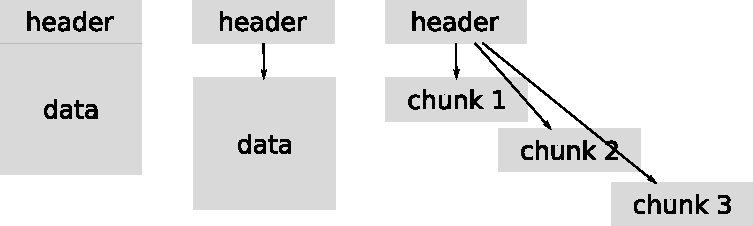
\includegraphics{data_layout.pdf}}
\caption{The three data layouts in \textit{DataSet}}
\label{fig:datalayout}
\end{figure}

If the data is sufficiently small \texttt{H5D\_COMPACT} will be used. In this layout the data address follows right after the header as shown on the left. When the data is larger but not growing, \texttt{H5D\_CONTIGUOUS} in the middle, is the right layout. This one allows the data to be located somewhere arbitrary in memory whereas a link is created into the header. The last layout, \texttt{H5D\_CHUNKED} on the right, is useful if the size of the data is unknown. The data will be divided into chunks with the same size where the address of each chunk will be stored in the header. This implies when a chunk is full a new one can be easily allocated and linked in the header, which is ideal for this project.
%bigger change
The goal is to store the time evolution of a matrix, a vector or simple values into one compact \textit{DataSet}. This can be achieved when the first dimension is reserved for time itself. Therefore a matrix has three dimension where the first dimension is for the time index $T_{index}$ and the others for row and column dimension respectively. Hence the chunk size in this case is defined by the matrix dimension and one chunk corresponds to the matrix belonging to a certain time index. The real time value can be calculated with the following formula:
\begin{equation}
\label{eq:mapping}
 T_{real} = T_{start} + T_{index} \cdot \Delta t
\end{equation}
This will be used in chapter \ref{chapt:datatest} to match data points between two \textit{H5Files} according to their transformed timegrids.

\section{DataType}
\label{seq:datatype}
The language C++ itself supports data types such as \emph{int}, \emph{double}, \emph{char} etc. but these cannot be used directly in a binary data format.
This is caused by the different data representations which are not homogeneous across different operating systems and system architectures. For example the difference between little-endian and big-endian machines. Thus the library has its own definitions which are compatible across platforms which are incorporated into the different classes as seen in figure \ref{graph:hierarchy}. It is intuitively clear from their names which classes must be used to describe which data types. For instance for writing floating point numbers the \textit{FloatType} class is used, where it also would be possible to change from IEEE representation to another one. In this project the \textit{PredType} and \textit{CompType} are the most relevant classes. From \textit{PredType}, which is predetermined through the C++ language, the \textit{NATIVE\_INT} type is utilized for writing timegrids. The \textit{CompType} class is used for
writing compositions of simple types such as a \textit{struct} of two \textit{doubles}. This is useful to construct a complex data type which will be explained in section \ref{seq:datatypedec}.

\section{DataSpace}
\label{seq:dataspace}
To describe the shapes of our data the \textit{DataSpace} class is required. The construction of such a \textit{DataSpace} is straightforward. First of all the library needs to know the number of dimensions of the desired space. Second it has to know the number of elements along each dimension. For the second argument an array of \texttt{hsize\_t} is expected instead of \texttt{int} as described in section \ref{seq:internaltypes}. To give the reader an idea the following code prepares the \textit{DataSpace} of a timegrid.

\begin{lstlisting}
int rank = 1;
hsize_t size[rank];
size[0] = number_of_timesteps;
DataSpace limited_timespace(rank,size);
\end{lstlisting}
The problem herein lies in the number of time steps which is known only at runtime. This leads to another approach which is to define a unlimited \textit{DataSpace}. The library allows this if an additional optional argument is added. This argument has to be of the same data type as the second argument and contains the maximum size of each dimension. The library expects that the values in this argument are greater or equal than in the previous argument otherwise an exception is thrown. For an unlimited space a special state is used namely \texttt{H5S\_UNLIMITED}. The above example code changes to the following if an unlimited space is desired:
\begin{lstlisting}
int rank = 1;
hsize_t size[rank] = {1};
hsize_t maxsize[rank] = {H5S_UNLIMITED};
DataSpace unlimited_timespace(rank, size, maxsize);
\end{lstlisting}

\section{PropList}
Most classes require a specific property list at the moment of construction which include additional information. Depending on the object a different property list is needed. All these lists have a common base class namely \textit{PropList} as presented in figure \ref{graph:hierarchy}. The possible applications of these property lists excel the scope of this project easily therefore the default value is enough. The default values are shortly described in table \ref{table:default}.

\begin{figure}[ht!]
\centering
\begin{tabular}{|l|l|}
\hline
Default name value&Influence\\
\hline
\texttt{H5P\_FILE\_CREATE}&\textit{H5FILE} creation\\
\texttt{H5P\_FILE\_ACCESS}&\textit{H5FILE} access\\
\texttt{H5P\_DATASET\_CREATE}&\textit{DataSet} creation\\
\texttt{H5P\_DATASET\_XFER}&raw data transfer\\
\texttt{H5P\_MOUNT}&\textit{H5File} mounting\\
\texttt{H5P\_DEFAULT}&base value for all the above\\
\hline
\end{tabular}
\caption{Table of property list default values and their influence}
\label{table:default}
\end{figure}

Noteworthy for this project is only the \textit{DSetCreatePropList} mentioned in section \ref{seq:dataset} which will be explained next.

\subsection{DSetCreatePropList}
\label{seq:dscpl}
From section \ref{seq:dataset} a \textit{DSetCreatePropList} object is demanded for creating a \textit{DataSet}. As the perceptive reader can guess this property list is used to determine the data layout shown in figure \ref{fig:datalayout}. The property list is responsible for setting the layout to \texttt{H5D\_CHUNKED}. This is important because only data with this layout can be dynamically extended later on during a simulation. 
\begin{lstlisting}
//create default H5P_DATASET_CREATE
DSetCreatePropList list;
//set chunked data layout
list.setChunk(int number_of_dim, hsize_t* dim);
//set the fill value after allocation
list.setFillValue(DataType type, void* default_value);
\end{lstlisting}
The above code configures a chunked layout into the property list for the construction of a \textit{DataSet}. Furthermore a default fill value can be defined which is utilized to fill newly allocated memory.

\section{Attribute}
\label{seq:attribute}
Additionally to writing simulation data in binary format it should also incorporate saving the corresponding simulation configuration. This can be easily done with \textit{Attributes} which must be attached to an affiliated \textit{Group} or \textit{DataSet}. The allocation of such an \textit{Attribute} is similar to a \textit{DataSet} meaning a \textit{DataType} and \textit{DataSpace} is also demanded. For its property list only the \texttt{H5P\_DEFAULT} is allowed which the library enforces otherwise an exception is thrown. For illustration see the subsequent code.
\begin{lstlisting}
Attribute attribute;
//group attribute
attribute = group.createAttribute(string "attributename",DataType type,DataSpace space,PropList plist);
//dataset attribute
attribute = dataset.createAttribute(string "attributename",DataType type,DataSpace space,PropList plist);
\end{lstlisting}

\chapter{Implementation}
\section{Link to Eigen library}
\label{seq:linkeigen}
As mentioned in the section \ref{seq:background} the simulation boils down to propagating the set $\Pi=\{ \vec{q},\vec{p},\mat{Q}, \mat{P},S\}$, where $\vec{q}$ and $\vec{p}$ are $D$ dimensional real-valued vectors, $\mat{Q}$ and $\mat{P}$ hold complex $D \times D$ matrices and $S$ is the global complex phase. A possible interface to work with these matrices and vectors is the \textit{Eigen} library \cite{eigenweb}. The simplified definition of an \textit{Eigen} matrix has the following form:
\begin{lstlisting}
Eigen::Matrix<complex<double>,row_dim,column_dim> mat;
\end{lstlisting}
Note that this is a class template over three parameters namely type, row-dimension and column-dimension. Therefore the overall implementation will also be a template. In the current version only scalar \textit{Hagedorn} wavepackets are supported thus only one dimension parameter $D$ is utilized but the framework can still easily be extended in the future. As discussed in section \ref{seq:datatype} native types are not writable, hence the type is defined through the library. This declared type is not necessarily the same as the template argument from \textit{Eigen}, but is still similar enough to permit basic transformation functions which are discussed in section \ref{seq:transform}.

\section{DataType Declaration}
\label{seq:datatypedec}
In this context simulation means manipulation of complex numbers. To build a \textit{DataType} the library needs access to its members thus the standard \texttt{complex} class cannot be utilized. Therefore a \texttt{struct} is most suitable for defining the fundamental structure since all its members are by default public accessible. Hence our declaration of complex numbers looks like this:
\begin{lstlisting}
struct ctype
{
  double real;
  double imag;
} instance_of_ctype;
\end{lstlisting}
This can now be used by the library to create the corresponding \textit{DataType}. In this case the \textit{CompType} is most suitable because \texttt{ctype} is a composition of simple data types. To be compatible with Python the same labels for its members have to be used which results in the following code:
\begin{lstlisting}
CompType hdfctype_(sizeof(instance_of_ctype));
hdfctype_.insertMember("r",HOFFSET(ctype,real), PredType::NATIVE_DOUBLE);
hdfctype_.insertMember("i",HOFFSET(ctype,imag), PredType::NATIVE_DOUBLE);
\end{lstlisting}
Worth noting is that the constructor of \textit{CompType} relies on the \texttt{sizeof} operator which tells how many bytes for an instance of this type are needed. The string labels "r" and "i" are utilized for the real respective the imaginary part of a complex number. \texttt{HOFFSET} is a simple macro which returns at which position counted in bytes the second argument is located inside the first argument. In this case the first \texttt{double}(real) is located at "0" and the second double(imag) at "8" since one \texttt{double} is $8$ Bytes long. Finally the last argument is the type inserted at this position. As already discussed in section \ref{seq:datatype} \texttt{double} cannot be used directly and the library provides compatible definitions through the \textit{PredType} class. The members of \textit{PredType} are constant and are fixed through the C++ language itself.\\

\section{Constructor}
\label{seq:ctor}
Since the data type declaration only has to be initialized once, it is suitable to pack it into the constructor of this writer template. The constructor only expects one string argument, namely the filename. Therefore the constructor can be written accordingly:
\begin{lstlisting}
template<int D>
...
//constructor
hdf5writer(string name):filename_(name), hdfctype_(sizeof(instance_of_ctype)), file_(filename_,H5F_ACC_TRUNC)
{
	hdfctype_.insertMember("r", HOFFSET(ctype,real), PredType::NATIVE_DOUBLE);
	hdfctype_.insertMember("i", HOFFSET(ctype,imag), PredType::NATIVE_DOUBLE);
}
\end{lstlisting}
Observe that there are two implicit constructor calls after instantiation of the filename. For the former refer to section \ref{seq:datatypedec} whereas for the latter see section \ref{seq:h5file}.

\section{Write options}
To enable customization about what and when something is written an additional layer was inserted. This was done with functions which set the desired configuration. In the current implementation there are three choices to make. By default writing \textit{Hagedorn} wavepackets is enabled, whereas writing the corresponding observables are disabled. This behavior is directed by a boolean. 
%bigger change
As already mentioned in section \ref{seq:dataset} for each chunk, which is in essence a matrix or vector, also the time index of the current time step is written in an additional \textit{DataSet}. These are shown in figure \ref{graph:file} where "timegrid" was used as its name. The corresponding customization thereof is to set the difference between two consecutive entries. More precisely, it is the choice if a \textit{DataSet} should be written in each time step ($d=1$) or every second time step ($d=2$) etc. The supported functions are listed subsequently:
\begin{lstlisting}
set_write_packet(true|false);
set_write_norm(true|false);
set_write_energies(true|false);
set_timestep_packet(1|2|3|...);
set_timestep_norm(1|2|3|...);
set_timestep_energies(1|2|3|...);
set_timestep_ekin(1|2|3|...);
set_timestep_epot(1|2|3|...);
\end{lstlisting}

\section{DataSet paths}
The structure and the names in figure \ref{graph:file} is fixed in the implementation as it is analogous to the hierarchy generated by the Python code. The data test is build on this structure as well. This can be problematic, once a change happens in the Python or C++ implementation, where the structure is affected. Luckily the library throws an \emph{invalid path} exception if such a change occurs and the paths are no longer valid. Future work could focus on making data test path independent for \textit{DataSets}.

\section{Prestructure}
\label{seq:prestructure}
This function is a bundle of steps which either have to be done prior to the writing process or are constant and therefore only need to be done once. The function definition is shown subsequently:
\begin{lstlisting}
template<class MultiIndex>
prestructuring(ScalarHaWp<D,MultiIndex> packet, double dt);
\end{lstlisting}
The dimension $D$ and the class \texttt{MultiIndex} are prerequisite for constructing a scalar \textit{Hagedorn} wavepacket and are detailed explained in the thesis of M. B\"osch \cite{bt_michajab}. A scalar \textit{Hagedorn} wavepacket includes a matrix of coefficients and the set $\Pi=\{ \vec{q},\vec{p},\mat{Q}, \mat{P},S\}$. The coefficient dimension is dependent on $D$ and \texttt{MultiIndex}, therefore the number of coefficients is calculated and stored first in this function. Next the \textit{Groups} of figure \ref{graph:file} are set up. Additionally some \textit{Attributes} are attached to the root group such as the time step $dt$. As discussed in section \ref{seq:dataset} each \textit{DataSet} has to be chunked according to a time step. Hence this chunk dimension is set in the next step for all \textit{DataSets} specified in the write options. E.g. for a packet the chunk-dimension for the coefficients, $\vec{q}$, $\vec{p}$, $\mat{Q}$, $\mat{P}$ and $S$ have to be set into an instance of \textit{DSetCreatPropList} individually. 
For instance a chunk-dimension of a $2 \times 2$ matrix in time is declared in the following form:
\begin{lstlisting}
hsize_t chunk[3] = {1,2,2};//{time_dim,row_dim,column_dim}
\end{lstlisting}
For further instruction see section \ref{seq:dscpl}. Before it is possible to allocate all \textit{DataSets} according to figure \ref{graph:file} also the individual \textit{DataSpaces} have to be declared. Luckily it is possible to reuse all chunk-arrays as arguments for their own \textit{DataSpace} with the additional array argument according to section \ref{seq:dataspace}. Now all building blocks are ready to allocate in the next step all \textit{DataSets}. It can be observed that there is a source and a destination \textit{DataSpace} with a corresponding selection in each time step. The destination \textit{DataSpace} grows over time within the file and thus is not constant. Different from the destination, the source \textit{DataSpace} and its selection is constant and therefore can be fixed in this step for the whole simulation. Notice that \textit{DataSpace} is the space of possible positions where data can be written to, whereas it needs to be specified which elements in \textit{DataSpace} are utilized. This is done with a selection which is described by a hyperslab and will be explained in the next section.

\section{Selection}
\label{seq:selection}
As already mentioned in the last section a selection within a \textit{DataSpace} is represented by a hyperslab. A hyperslab consists of four arrays namely:
\begin{lstlisting}
hsize_t start[3] = {time_index,1,1};
hsize_t count[3] = {time_index,3,2};
hsize_t block[3] = {time_index,1,1};
hsize_t stride[3] = {time_index,2,2};
\end{lstlisting}
Notice that the first dimension is always reserved for the time dimension. The implementation has an internal index for storing the current simulation step which is used as the label. Thus only the index for the next time step has to be incremented without altering the code for the selection. The following figure \ref{fig:hyperslab} illustrates why four arrays are required to represent a hyperslab.

\begin{figure}[ht!]
\centering
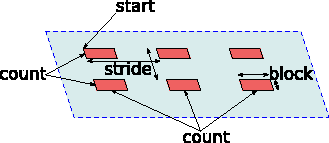
\includegraphics[scale=1.8]{selection.pdf}
\caption{hyper-slab illustration}
\label{fig:hyperslab}
\end{figure}
In figure \ref{fig:hyperslab} the blue dashed plane symbolizes a matrix in three dimensions. The first dimension is reserved for time meaning the blue dashed plane depicts a matrix at some point in time. One red block represents one single element in this matrix. Thus this figure displays the hyperslab from the previous code segment. The selection is done by the \textit{DataSpace} itself whereas the \texttt{H5S\_SELECT\_SET} argument is recommended to overwrite the old selection.
\begin{lstlisting}
dataspace.selectHyperslab(H5S_SELECT_SET, count, start, stride, block);
\end{lstlisting}
In case a contiguous block of data is written the last two arguments can be omitted.
\begin{lstlisting}
dataspace.selectHyperslab(H5S_SELECT_SET, count, start);
\end{lstlisting}


\section{Transformation}
\label{seq:transform}
As indicated in section \ref{seq:linkeigen} basic transformations are applied to the \textit{Eigen} matrices. The internal data of an \textit{Eigen} matrix can be extracted with the \texttt{matrix.data()} function. Either the data is of type \texttt{complex<double>} or \texttt{double} which can be transferred to \texttt{ctype}. From \texttt{complex<double>} its members can be simply copied over whereas for a \textit{double} the imaginary part is simply set to zero. After this step all data originally saved in an \textit{Eigen} matrix are now stored in vectors of type \texttt{ctype}. Later on the data is again extracted with the \texttt{vector.data()} function and passed on to the HDF library for writing. The reason for this transformation from \texttt{complex<double>} or \texttt{double} to \texttt{ctype} is that in the actual writing function call \texttt{hdfctype\_} will be used as type argument. Since \texttt{hdfctype\_} is constructed from \texttt{ctype}, see section \ref{seq:ctor}, it can be safely assumed that the library can write pointers of type \texttt{ctype}.

\section{Writing}
\label{seq:writing}
All tools are ready to look at the actual writing function call for \textit{DataSets} and \textit{Attributes}:
 
\begin{lstlisting}
dataset.write(void* src, DataType type, DataSpace srcspace, DataSpace dstspace);
attribute.write(DataType type, void* src);
\end{lstlisting}
Notable is that the size of \texttt{src} is hidden in the selection of \texttt{srcspace}. Furthermore the destination is implicitly given by the \texttt{datasetname} where the function call occurred. When the selection of \texttt{srcspace} and \texttt{dstspace} does not match in size an exception is thrown. There are only two types used as \textit{DataType}. For simulation data \texttt{hdfctype\_} is utilized and for timegrids \texttt{PredType::NATIVE\_INT} is used. Remember also that all \texttt{srcspaces} are constant and therefore constructed in section \ref{seq:prestructure}.

\section{Extension}
\label{seq:extension}
The \textit{DataSets} in section \ref{seq:dataset} were explicitly constructed such that they have a chunked memory layout. This is useful now because the library can only extend this type of layout with the succeeding function call: 
\begin{lstlisting}
dataset.extend(hsize_t* dimension);
\end{lstlisting}
The new dimension is as expected an array of \texttt{hsize\_t} where there are two effects. When an entry in the array is smaller than the \textit{DataSet} itself, it will get shrunk along this direction. Alternatively if an entry is larger than the \textit{DataSet} itself, it will get extended along this direction. There will be no effect in case the argument is of the same size as the \textit{DataSet} itself. It is obvious that the \textit{DataSets} in this project only grow in the direction of time per construction. Thereby the chunk dimension can be reused except for the first(time) entry. For this entry an index for each individual \textit{DataSet} is utilized to keep track of the current size. Bear in mind that this index is not the same as the current time index which is used to write timegrids.

\section{Update}
\label{seq:update}
Naturally since all \textit{DataSets} were extended the corresponding \textit{DataSpace} used as the destination is invalidated. Furthermore each individual index used to keep track of the number of chunks used in section \ref{seq:extension} has to be incremented. Conveniently the HDF library provides a function to extract the \textit{DataSpace} from a \textit{DataSet} namely:
\begin{lstlisting}
DataSpace newdataspace = dataset.getSpace();
\end{lstlisting}
Now all outdated \textit{DataSpaces} are updated with the help of the extended \textit{DataSets}. This function also represents the last action done in the current time step. All actions from section \ref{seq:selection} to \ref{seq:update} are repeated in each time step of the simulation. Remember that the transformation is included because in each time step the \textit{Hagedorn} wavepacket is propagated according to the chosen scheme and thus was modified.

\section{Poststructure}
\label{seq:poststructure}
After the time loop of the simulation has ended it is important to finalize all structures from the library. Furthermore the last extension has to be reversed since no further data will be written. This is easily done with the same function but with a smaller index as explained before in \ref{seq:update}. All variables allocated on the stack are deleted automatically and thus can be neglected. The others allocated on the heap with the \texttt{new} operator need to be freed manually. Sensibly in this project all these pointer objects are forwarded to the standard library through the \texttt{shared\_ptr} container. Likewise \texttt{vector} is managed also by the standard library and thus the standard library guarantees that these objects will be freed correctly.

\section{Simulation in a picture}
The functionality of this writer template can be easily visualized when only one \textit{DataSet} is considered, see figure \ref{fig:illustration}.
\begin{figure}[ht!]
\resizebox{\textwidth}{!}{
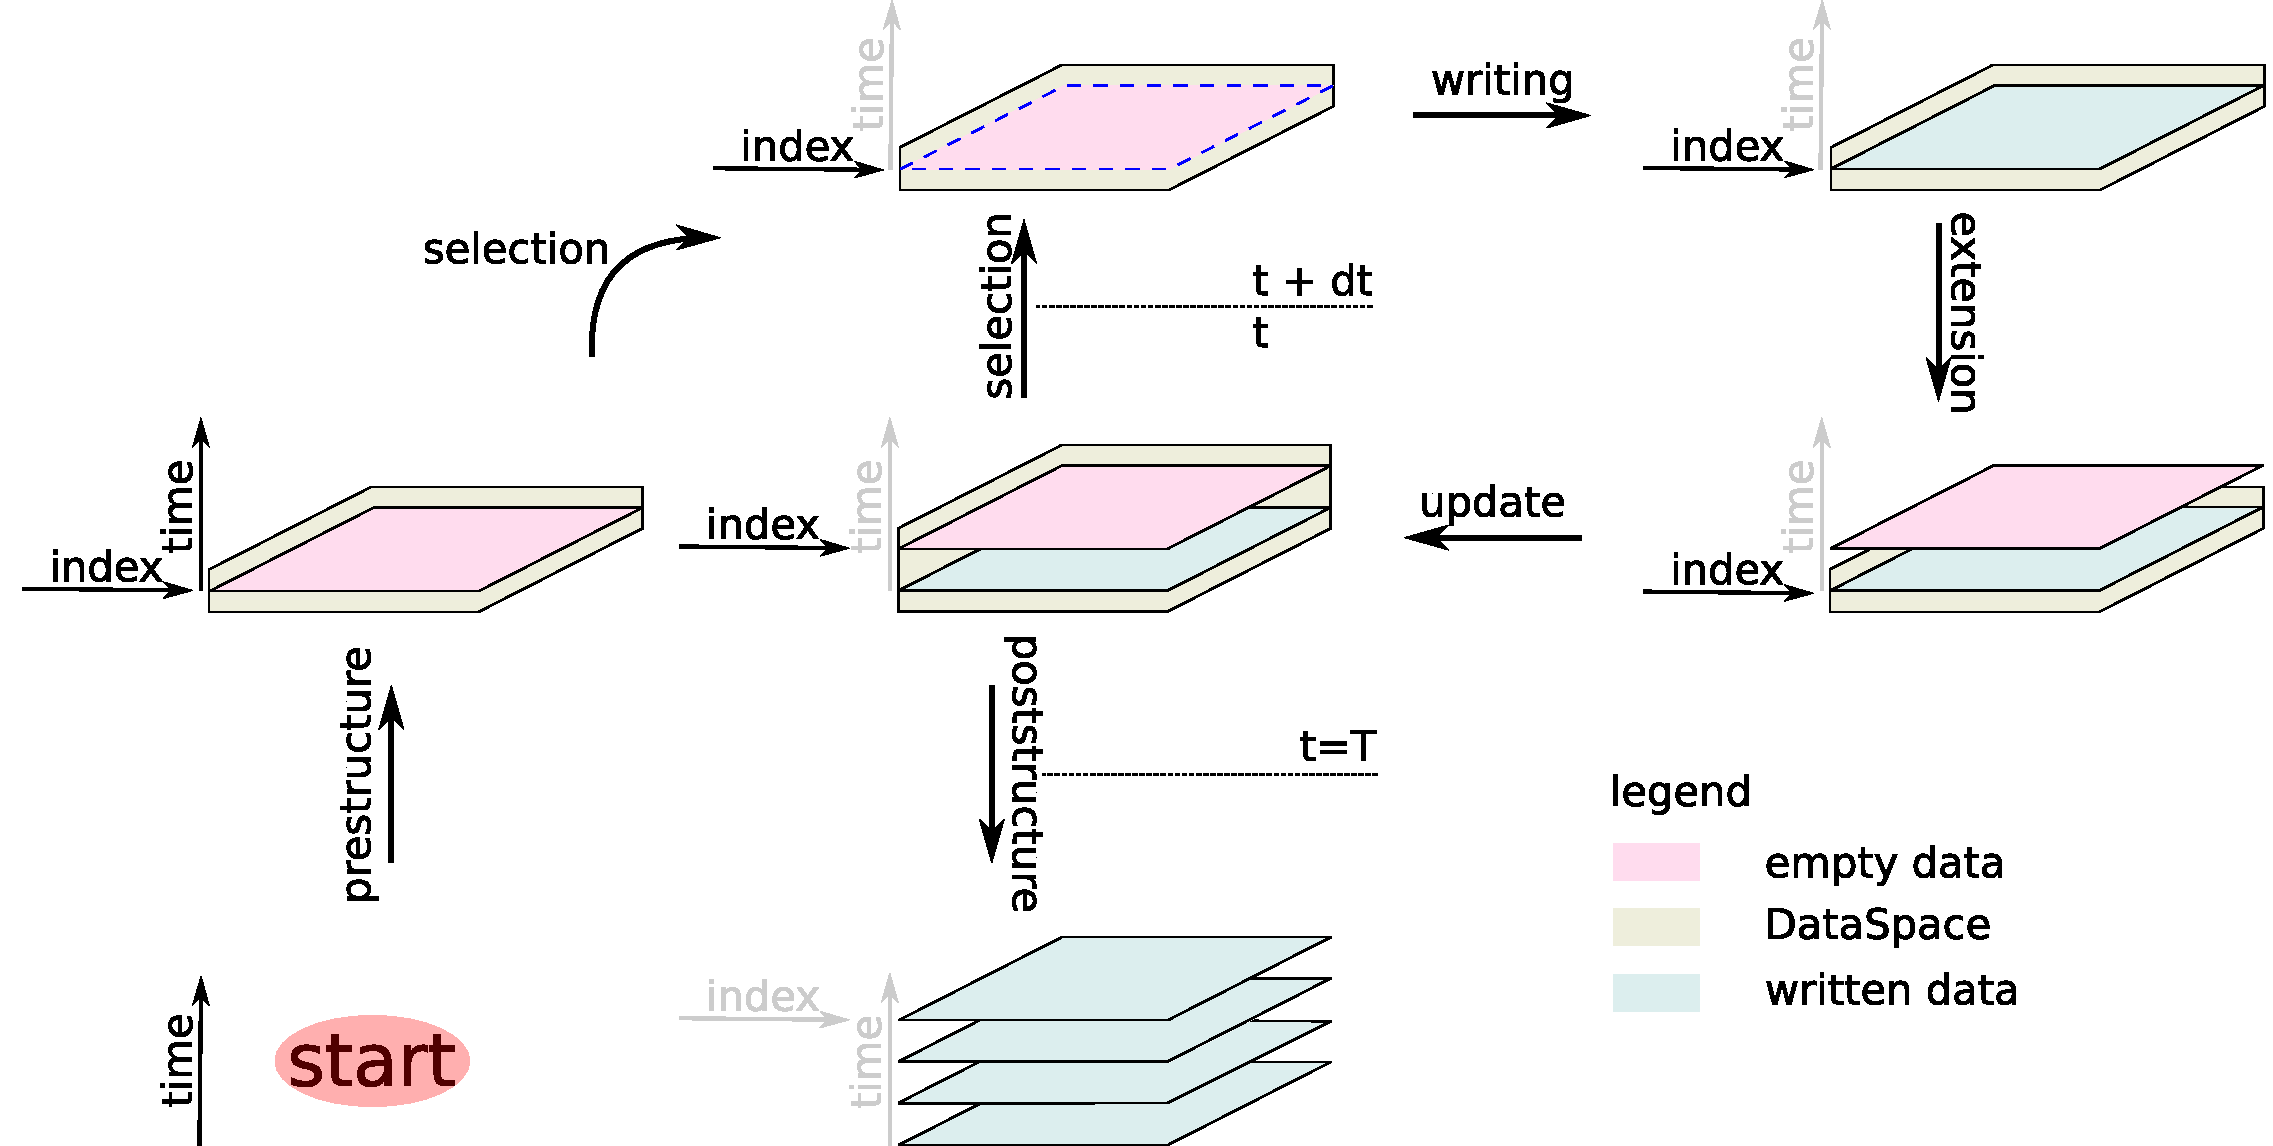
\includegraphics[scale=1.0]{writing_dataset.pdf}
}
\caption{Illustration of inner workings for a \textit{DataSet} in the simulation}
\label{fig:illustration}
\end{figure}
The start symbolizes the constructor of this class. The cycle begins with the selection process which sets a hyperslab, indicated by the blue dashed line. The sections \ref{seq:selection} through \ref{seq:update} are part of this cycle which halts only when the time step arrived at $T$. Then the simulation gets finalized with the poststructure function as described in section \ref{seq:poststructure}.

\section{Usage in Simulation}
The following code snippet shows how to use the key functionality of this class for writing \textit{Hagedorn} wavepackets:

\begin{lstlisting}
//Simulation settings
...
io::hdf5writer<D> writer("simulation_filename.hdf5");

writer.prestructuring<MultiIndex>(packet, dt);

//Time loop(propagation)
for(real_t t = 0; t < T; t += dt)
{
	//Write wavepacket
	writer.store_norm(packet);
	
	//Propagate wavepacket
   	propagator.propagate(packet, dt, V);
}

writer.poststructuring();
\end{lstlisting}
A more detailed version can be found in the appendix. The ellipsis there is fully expended and show how to generate the simulation setting for a harmonic $2D$ oscillator. To understand the simulation set up the reader can consult the preceding works online \cite{bt_michajab}, \cite{st_benedekv} and \cite{bt_lionelm} and the documentation therein. Furthermore additional information can be found in the documentation of the C++ implementation \cite{libwaveblocks}.

\chapter{Data Test}
\label{chapt:datatest}

\section{Introduction to GoogleTest}
There are two main ways to test objects with \textit{GoogleTest}. For the interested reader a more detailed description can be found in the git repository \cite{googletestdoc}, where the \emph{Primer.md} and \emph{AdvancedGuide.md} examples are strongly suggested. Of importance is to define a test class for reusing certain objects for all tests. These objects in this case are the two \textit{H5Files}, the \textit{DataType} used in the writing process and the \textit{Attributes} saved in the root group of the two files. One of these \textit{Attributes} is the time step $\Delta t$ utilized for the data matching. When there are two files in general they do not have necessarily the same time step size. However, mapped with the corresponding timegrid according to equation \ref{eq:mapping}, some of the data map to the same timepoint, and therefore can be compared. This is carried out by a function at the beginning, which tests if two \textit{DataSets} have matching timepoints, which will be stored in a list. If the list is empty a message will be printed and the program continues with the next \textit{DataSet}.

\section{The Main File}
\label{seq:testmain}
The main file consists of the test class for the shared objects, all test fissures which are based on the test class and the main function which invokes the test itself. The subsequent code snipped shows the core of the data test:

\begin{lstlisting}
#include "gtest/gtest.h"
int global_argc;
char** global_argv;
#define abstol 1e-6
...

class TestHDF : public ::testing::Test
{
	protected:
	TestHDF();
	virtual ~TestHDF();
	void SetUp();
	void TearDown();
	void time_matching(...);
	
	struct ctype{...};
	H5File cppfile;
	H5File pyfile;
	CompType hdfctype_;
	double dt_cpp;
	double dt_py;
	...
};

TEST_F(TestHDF, Testpacket)
{...}
TEST_F(TestHDF, Testenergies)
{...}
TEST_F(TestHDF, Testnorm)
{...}

int main(int argc,char* argv[])
{
	global_argc = argc;
	global_argv = argv;
	::testing::InitGoogleTest(&argc, argv);
	return RUN_ALL_TESTS();
}
\end{lstlisting}
First the \textit{TestHDF} class gets constructed where we use global \texttt{argc} and \texttt{argv} arguments to transfer the filenames from the console to the class. Notice also that \textit{TestHDF} needs to derive from \texttt{::testing::Test} from \textit{GoogleTest} to work. Then in the main function the test fissures are invoked with the \texttt{RUN\_ALL\_TESTS()} call. For a test fissure \texttt{TEST\_F()} an additional \texttt{SetUp()} function is provided for further specifying test settings. Afterwards each test fissure also gets cleaned up with the \texttt{TearDown()} function. In the test fissure itself the data test takes place. First the time matching function is invoked with the timegrids of both files as arguments. If the prepared list is not empty then the correct values are loaded from the \textit{H5Files}. These values are then compared with the \texttt{EXPECT\_NEAR(...)} function provided by the test framework which compares the difference of two \textit{doubles} to an absolute tolerance. This process will be repeated for each matching \textit{DataSet} in these two files until non-zero return code in \texttt{RUN\_ALL\_TESTS()} finish the execution. If the difference between two \textit{doubles} is larger than the defined absolute tolerance they will be printed out automatically and the test will proceed.

\chapter{Conclusion}
This project successfully implemented a more sophisticated way to serialize \textit{Hagedorn} wavepackets using the HDF5 C++ interface. Hereby the dependence on an external project \cite{eigen3-hdf5} was removed. This implementation handles \textit{Eigen} matrices by transforming the actual data, where complicated type derivation was also eliminated. This was achieved by adapting the type and hierarchy of the data for all simulations to the structure used by the Python code. This further allowed us to implement a data test, which based on type and hierarchy, can compare C++ and Python generated data. Though a user of the software \cite{libwaveblocks} has to be now aware that additionally to a compiler, which supports C++11 features, also \textit{Eigen}, \textit{HDF5} and \textit{GoogleTest} have to be installed. Hopefully this does not prevent some users to use \cite{libwaveblocks} since extra effort is required to install those libraries.

%\section{Outlook}



\appendix

\appendix

\section{Energy Evolution and Drift Plots}

\begin{figure}[ht]
	\centering
	\begin{minipage}[c]{\textwidth}
		\begin{center}
			\large Hagedorn Propagator \\[1mm]
			\normalsize Energy Evolution and Drift
			\vspace{4mm}
		\end{center}
	\end{minipage}
	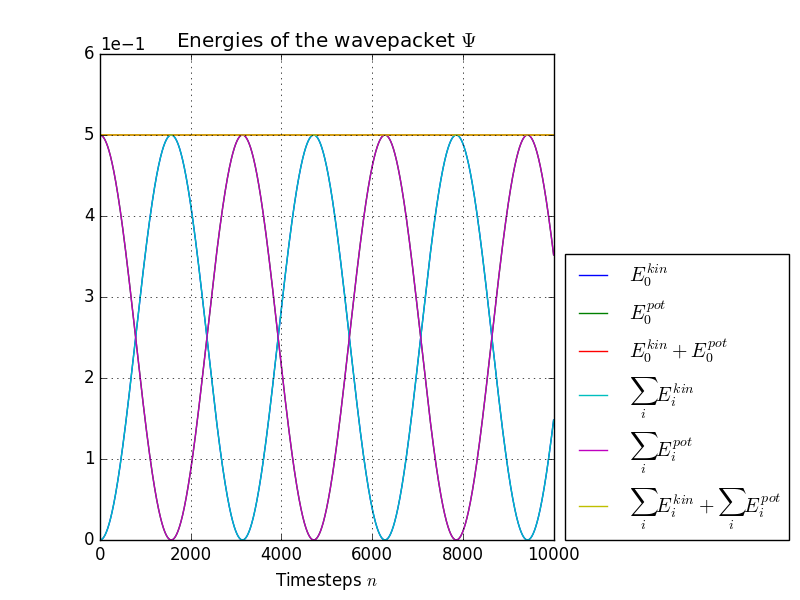
\includegraphics[width=.45\textwidth]{figures/harmonic_1D_Hagedorn_energies.png}
	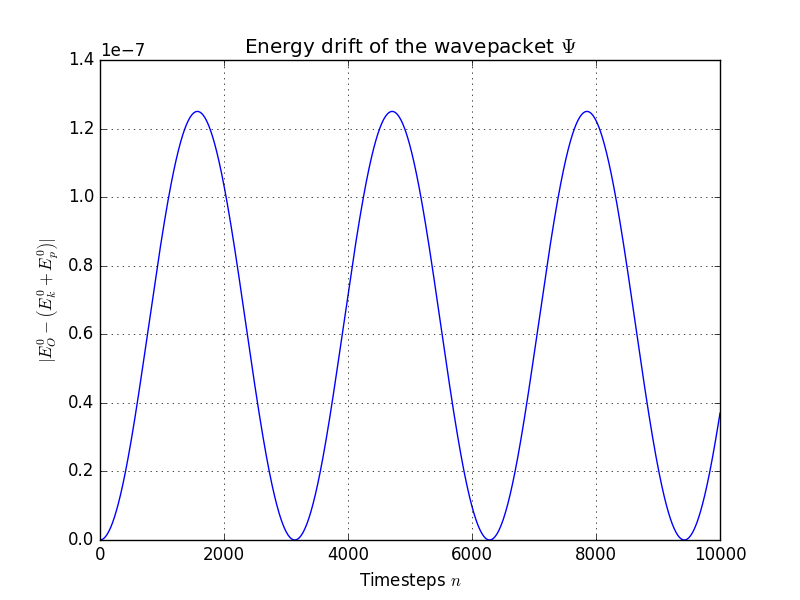
\includegraphics[width=.45\textwidth]{figures/harmonic_1D_Hagedorn_drift.png} \\
	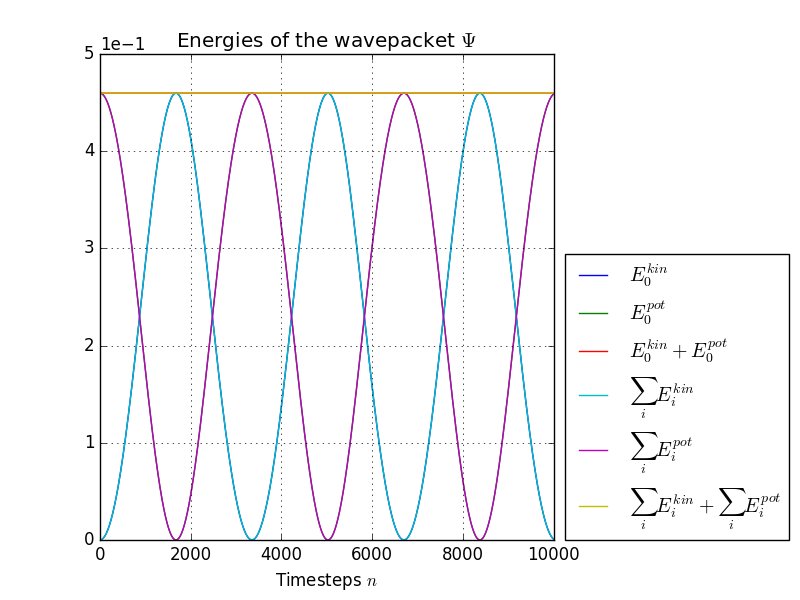
\includegraphics[width=.45\textwidth]{figures/torsional_1D_Hagedorn_energies.png}
	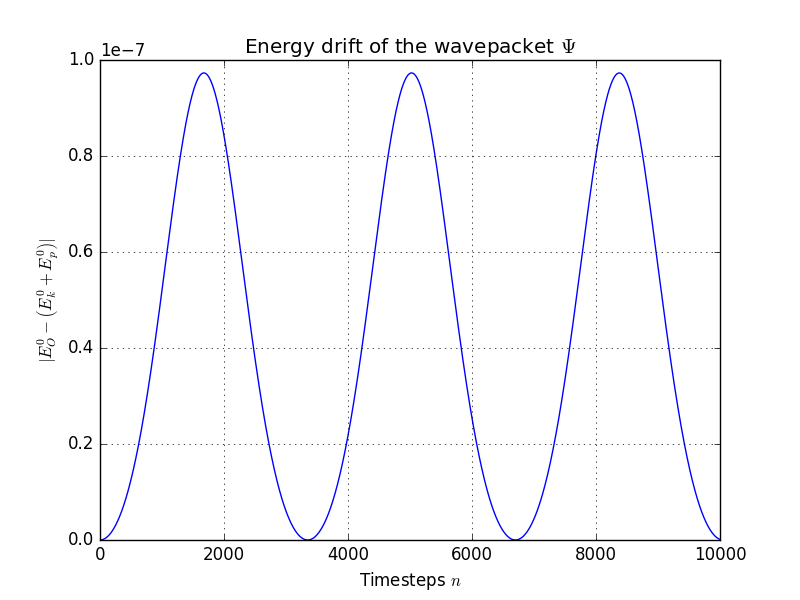
\includegraphics[width=.45\textwidth]{figures/torsional_1D_Hagedorn_drift.png} \\
	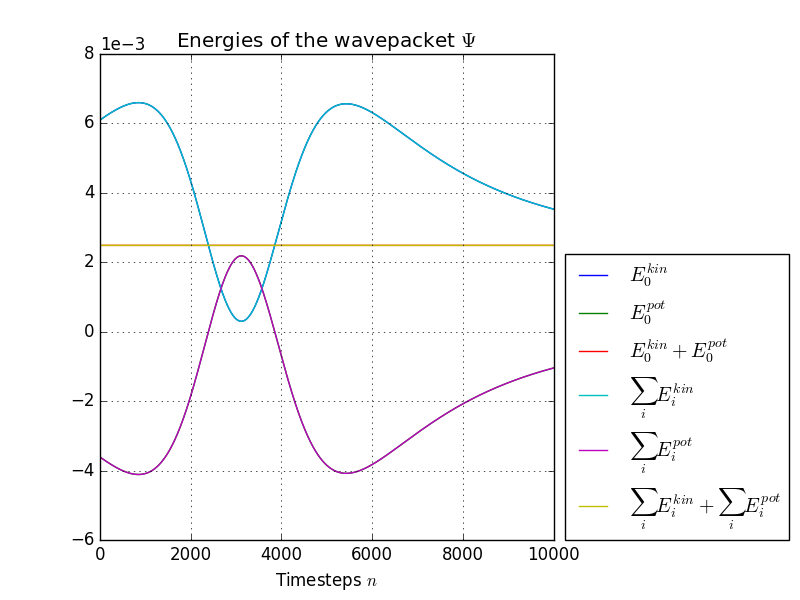
\includegraphics[width=.45\textwidth]{figures/morse_1D_Hagedorn_energies.png}
	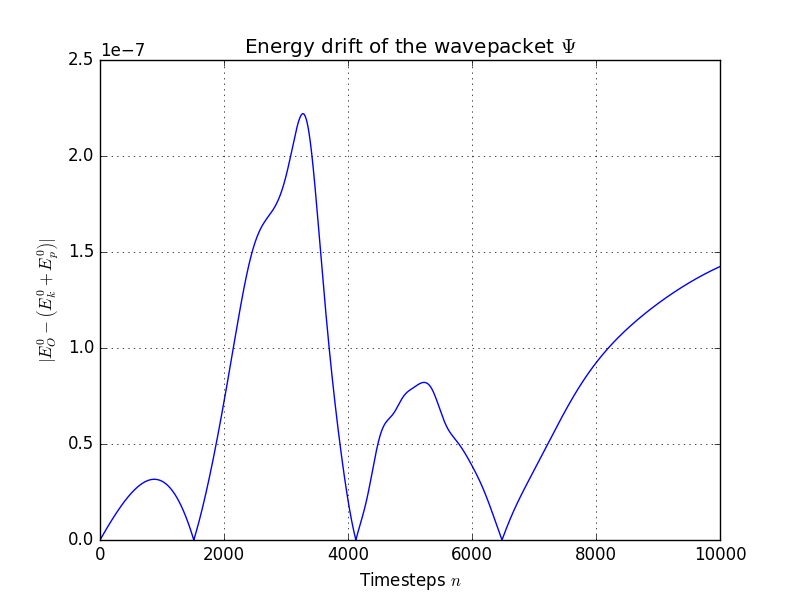
\includegraphics[width=.45\textwidth]{figures/morse_1D_Hagedorn_drift.png}
	\caption{Energy evolution and drift for a 1D wave packet propagated with the Hagedorn propagator in a harmonic potential (top), a torsional potential (middle) and a Morse potential (bottom).
	(Parameters: $N=1$, $D=1$ $|\K|=16$ $\eps=0.01$ (Morse $0.0484$), $T=10$ (Morse $T=50$), $\Dt=0.001$ (Morse $\Dt=0.005$), Hagedorn propagator)}
	\label{fig:energy_Hagedorn}
\end{figure}
%
\begin{figure}[ht]
	\centering
	\begin{minipage}[c]{\textwidth}
		\begin{center}
			\large MG4 Propagator \\[1mm]
			\normalsize Energy Evolution and Drift
			\vspace{4mm}
		\end{center}
	\end{minipage}
	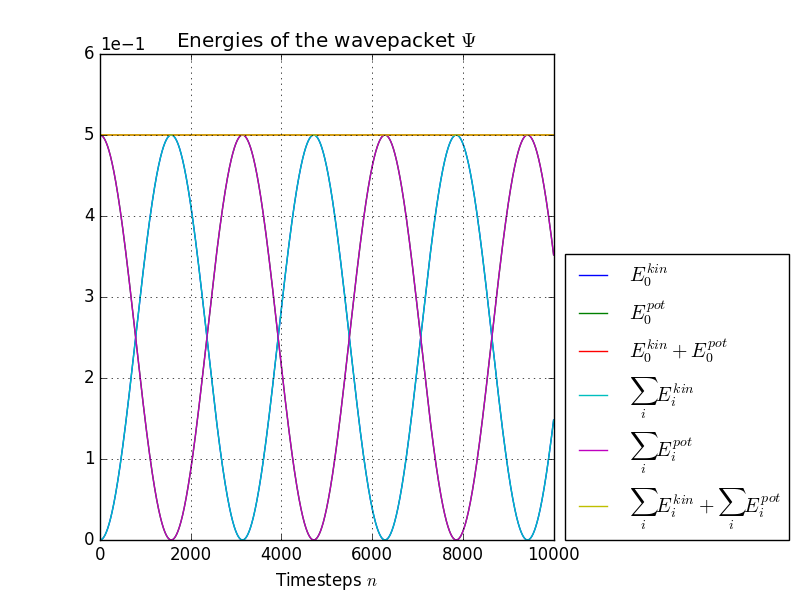
\includegraphics[width=.45\textwidth]{figures/harmonic_1D_MG4_energies.png}
	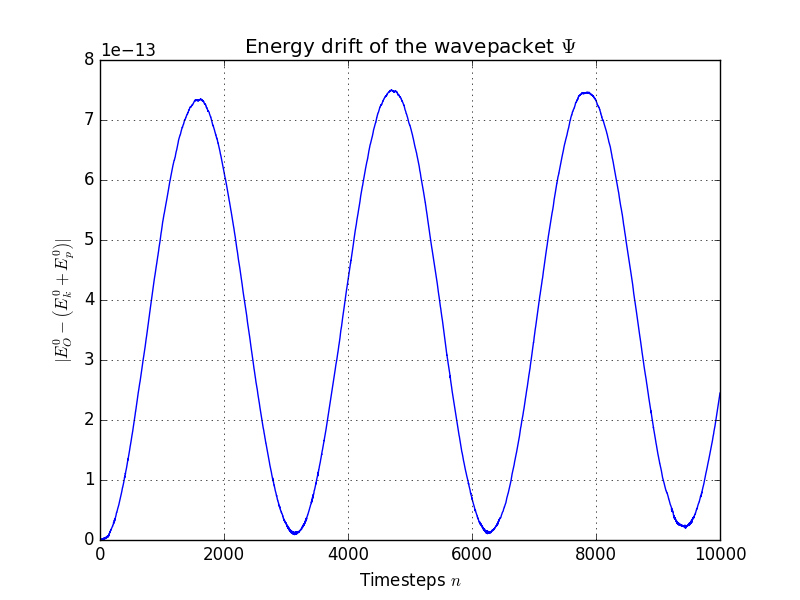
\includegraphics[width=.45\textwidth]{figures/harmonic_1D_MG4_drift.png} \\
	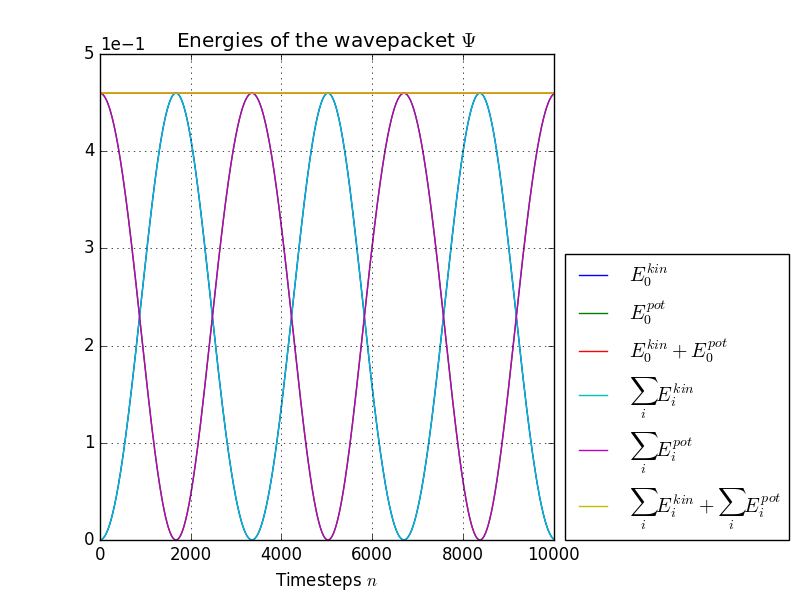
\includegraphics[width=.45\textwidth]{figures/torsional_1D_MG4_energies.png}
	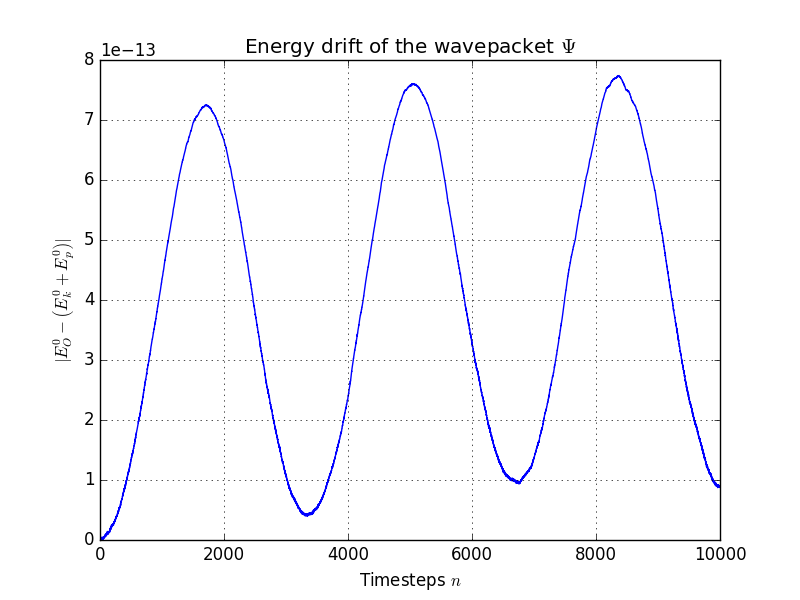
\includegraphics[width=.45\textwidth]{figures/torsional_1D_MG4_drift.png} \\
	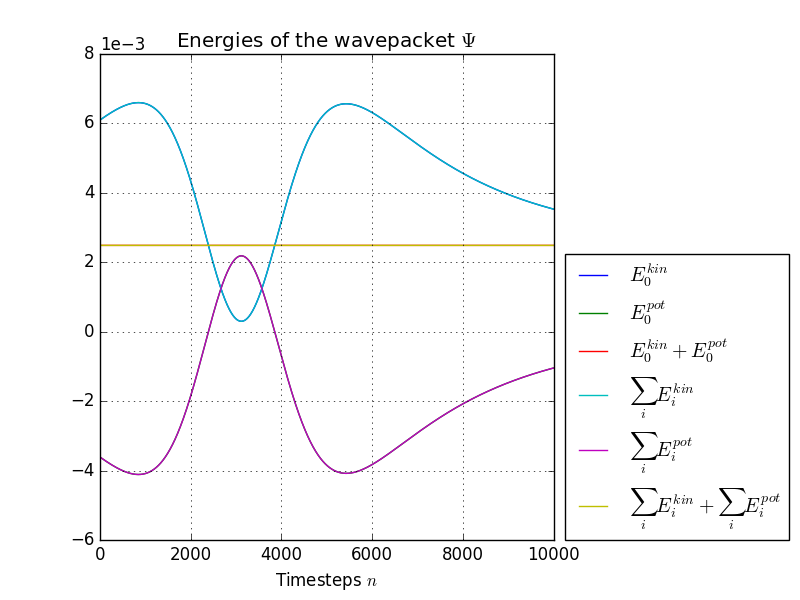
\includegraphics[width=.45\textwidth]{figures/morse_1D_MG4_energies.png}
	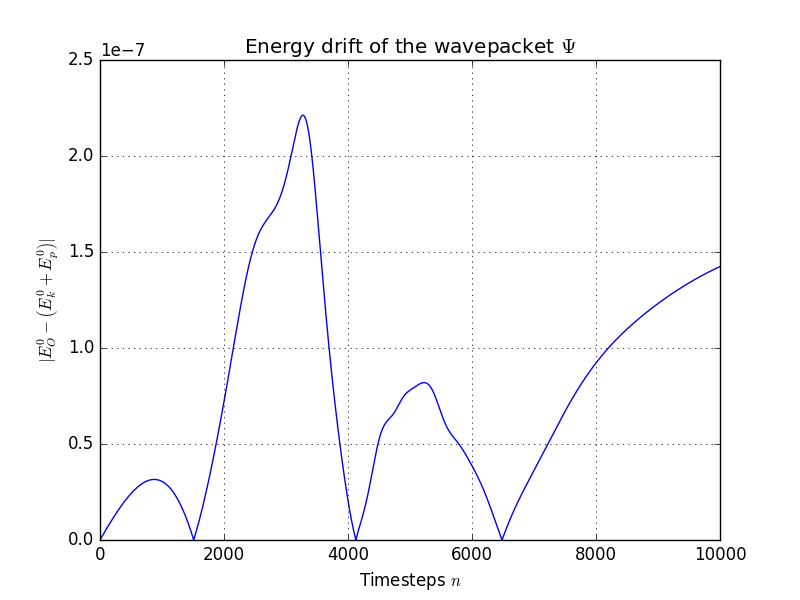
\includegraphics[width=.45\textwidth]{figures/morse_1D_MG4_drift.png}
	\caption{Energy evolution and drift for a 1D wave packet propagated with the MG4 propagator in a harmonic potential (top), a torsional potential (middle) and a Morse potential (bottom).
	(Parameters: $N=1$, $D=1$ $|\K|=16$ $\eps=0.01$ (Morse $0.0484$), $T=10$ (Morse $T=50$), $\Dt=0.001$ (Morse $\Dt=0.005$), MG4 propagator with \emph{Y4} splitting for \proc{IntSplit})}
	\label{fig:energy_MG4}
\end{figure}
%
\begin{figure}[ht]
	\centering
	\begin{minipage}[c]{\textwidth}
		\begin{center}
			\large McL42 Propagator \\[1mm]
			\normalsize Energy Evolution and Drift
			\vspace{4mm}
		\end{center}
	\end{minipage}
	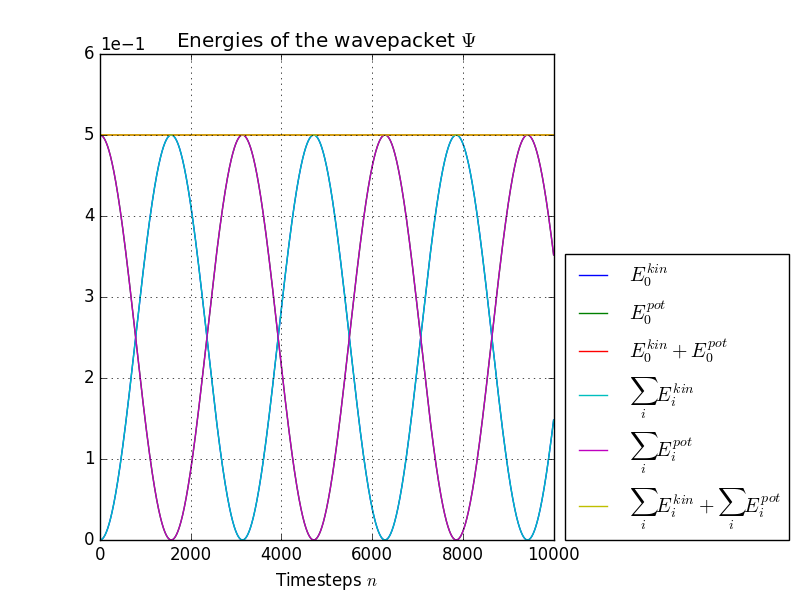
\includegraphics[width=.45\textwidth]{figures/harmonic_1D_McL42_energies.png}
	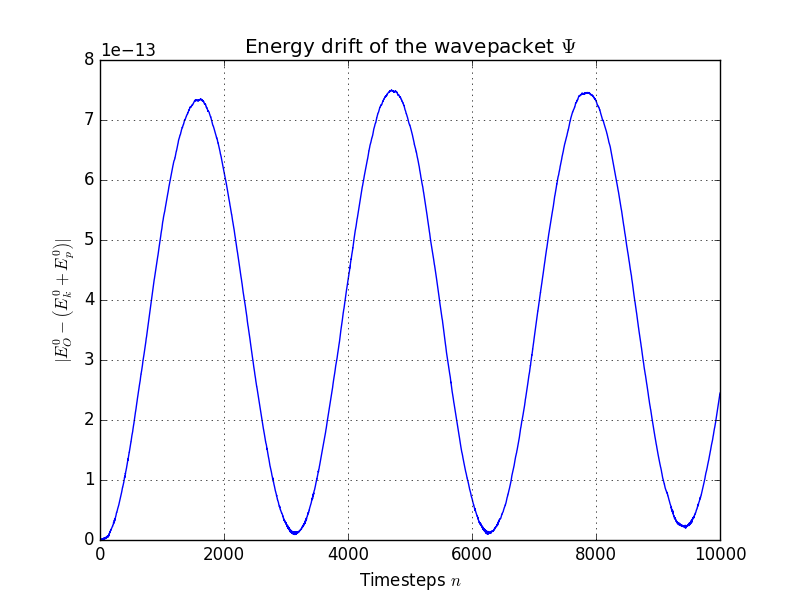
\includegraphics[width=.45\textwidth]{figures/harmonic_1D_McL42_drift.png} \\
	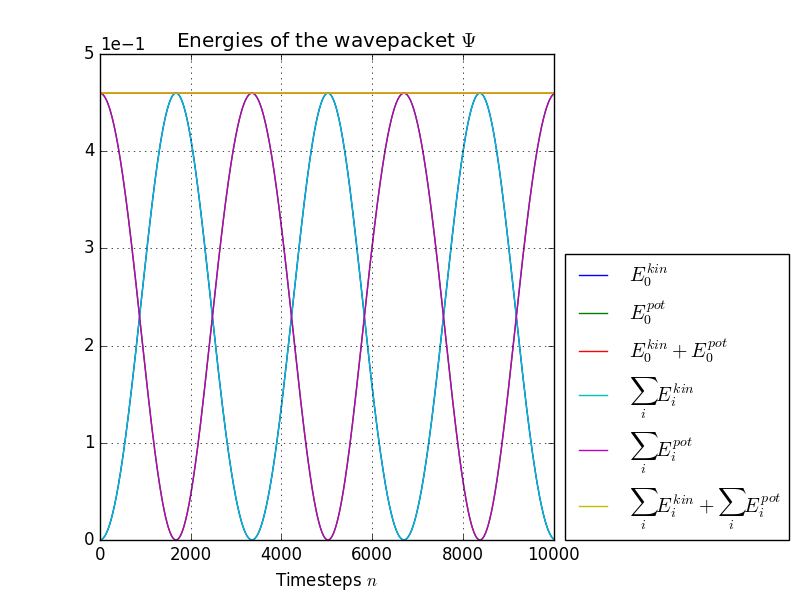
\includegraphics[width=.45\textwidth]{figures/torsional_1D_McL42_energies.png}
	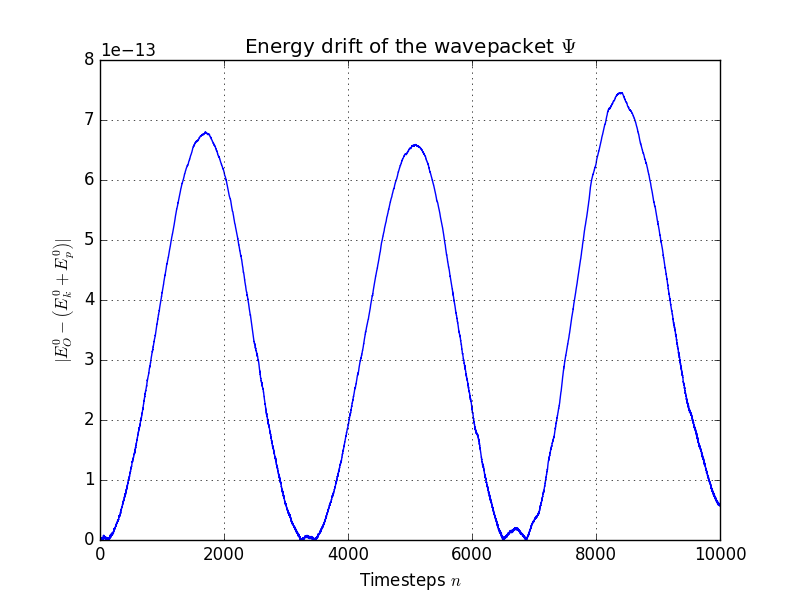
\includegraphics[width=.45\textwidth]{figures/torsional_1D_McL42_drift.png} \\
	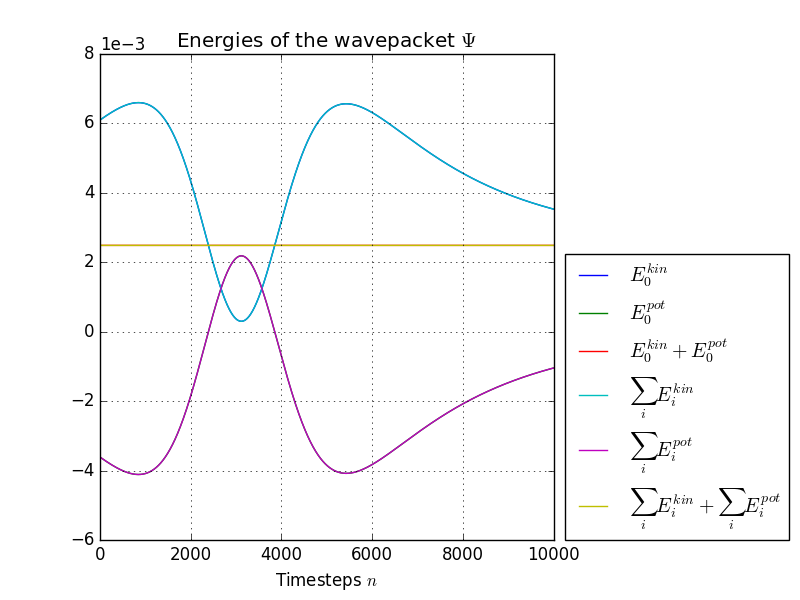
\includegraphics[width=.45\textwidth]{figures/morse_1D_McL42_energies.png}
	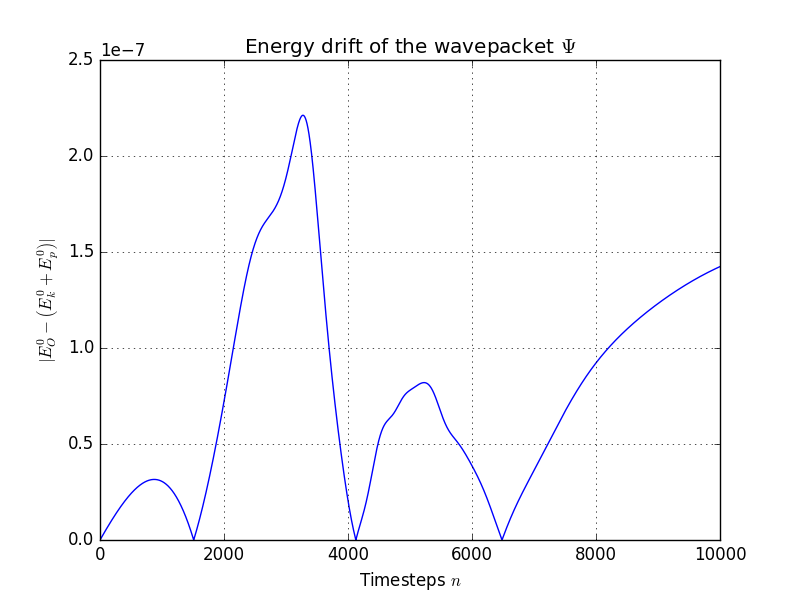
\includegraphics[width=.45\textwidth]{figures/morse_1D_McL42_drift.png}
	\caption{Energy evolution and drift for a 1D wave packet propagated with the McL42 propagator in a harmonic potential (top), a torsional potential (middle) and a Morse potential (bottom).
	(Parameters: $N=1$, $D=1$ $|\K|=16$ $\eps=0.01$ (Morse $0.0484$), $T=10$ (Morse $T=50$), $\Dt=0.001$ (Morse $\Dt=0.005$), McL42 propagator with \emph{Y4} splitting for \proc{IntSplit})}
	\label{fig:energy_McL42}
\end{figure}
%
\begin{figure}[ht]
	\centering
	\begin{minipage}[c]{\textwidth}
		\begin{center}
			\large McL84 Propagator \\[1mm]
			\normalsize Energy Evolution and Drift
			\vspace{4mm}
		\end{center}
	\end{minipage}
	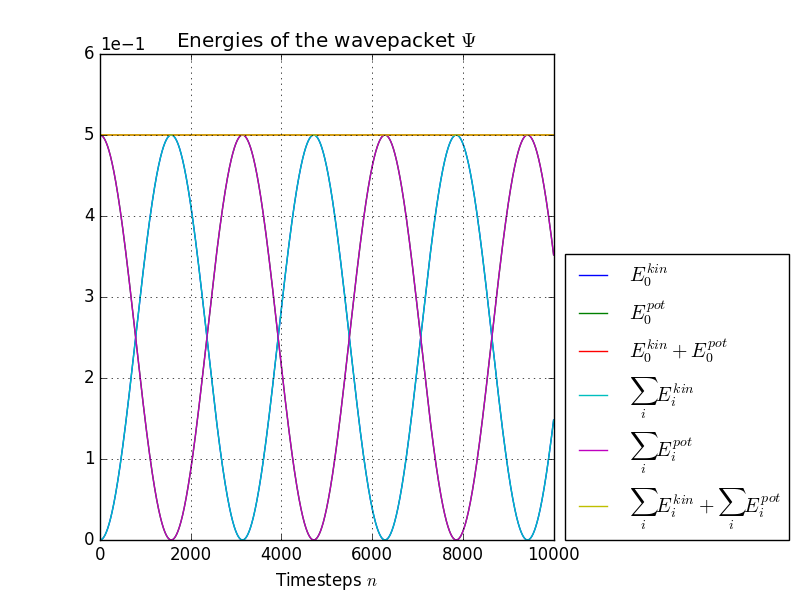
\includegraphics[width=.45\textwidth]{figures/harmonic_1D_McL84_energies.png}
	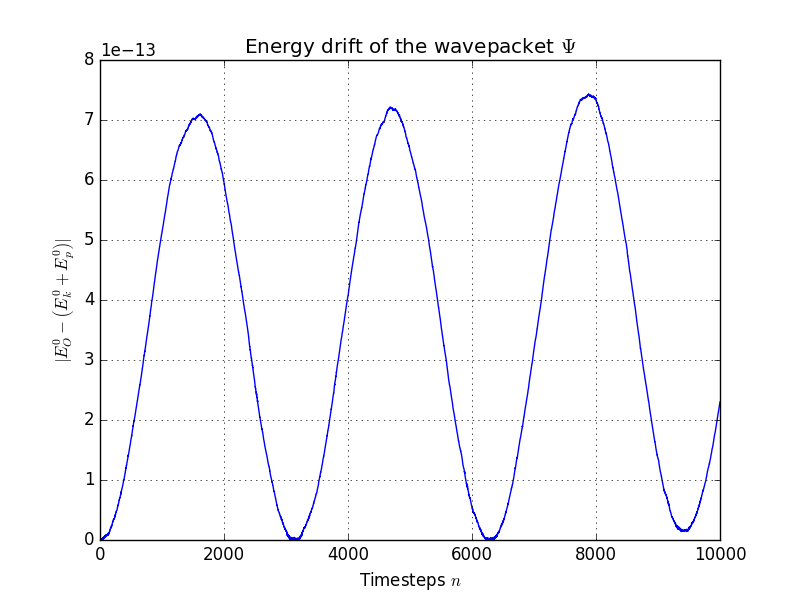
\includegraphics[width=.45\textwidth]{figures/harmonic_1D_McL84_drift.png} \\
	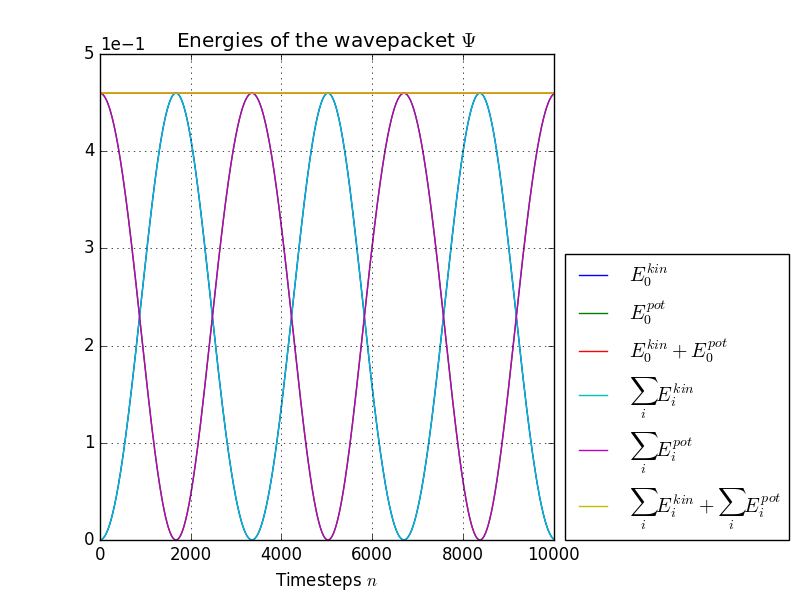
\includegraphics[width=.45\textwidth]{figures/torsional_1D_McL84_energies.png}
	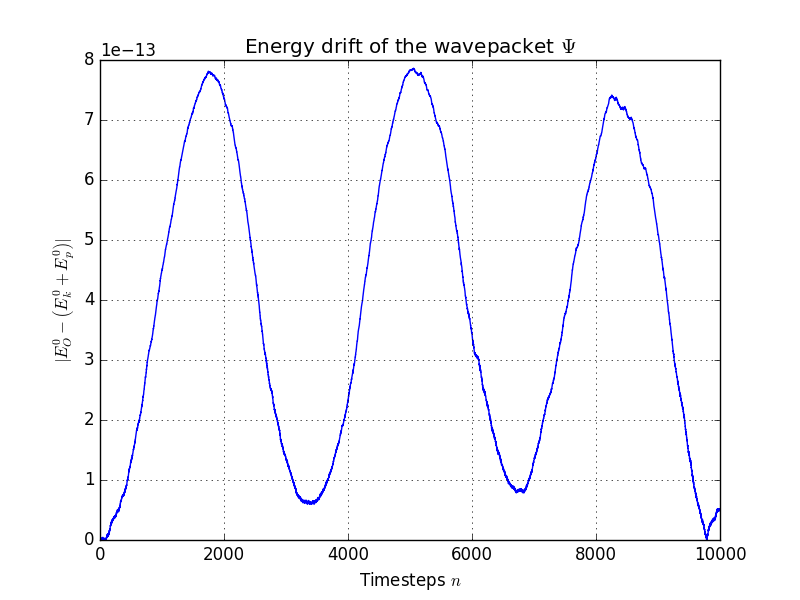
\includegraphics[width=.45\textwidth]{figures/torsional_1D_McL84_drift.png} \\
	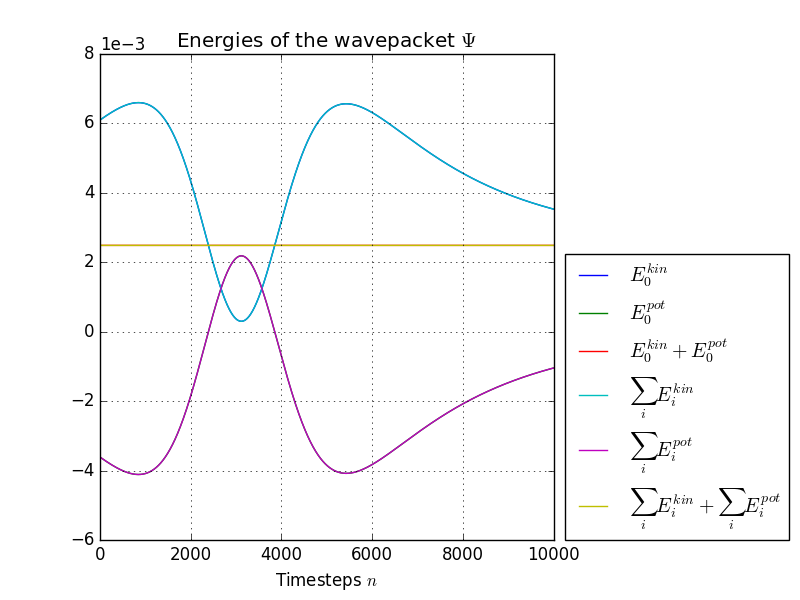
\includegraphics[width=.45\textwidth]{figures/morse_1D_McL84_energies.png}
	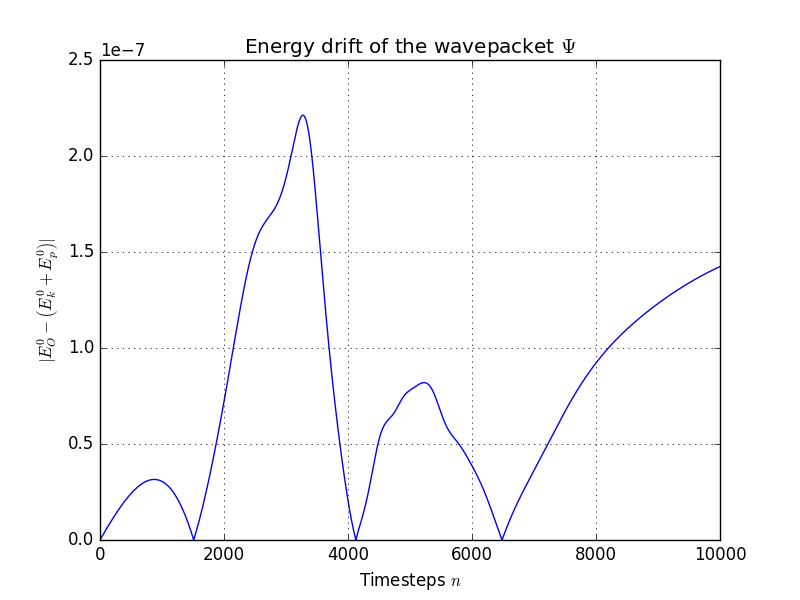
\includegraphics[width=.45\textwidth]{figures/morse_1D_McL84_drift.png}
	\caption{Energy evolution and drift for a 1D wave packet propagated with the McL84 propagator in a harmonic potential (top), a torsional potential (middle) and a Morse potential (bottom).
	(Parameters: $N=1$, $D=1$ $|\K|=16$ $\eps=0.01$ (Morse $0.0484$), $T=10$ (Morse $T=50$), $\Dt=0.001$ (Morse $\Dt=0.005$), McL84 propagator with \emph{Y4} splitting for \proc{IntSplit})}
	\label{fig:energy_McL84}
\end{figure}
%
\begin{figure}[ht]
	\centering
	\begin{minipage}[c]{\textwidth}
		\begin{center}
			\large Pre764 Propagator \\[1mm]
			\normalsize Energy Evolution and Drift
			\vspace{4mm}
		\end{center}
	\end{minipage}
	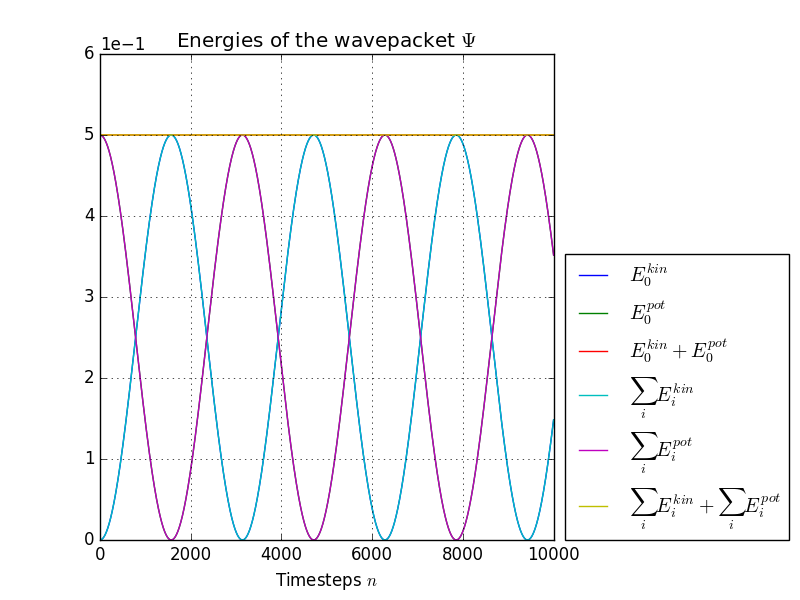
\includegraphics[width=.45\textwidth]{figures/harmonic_1D_Pre764_energies.png}
	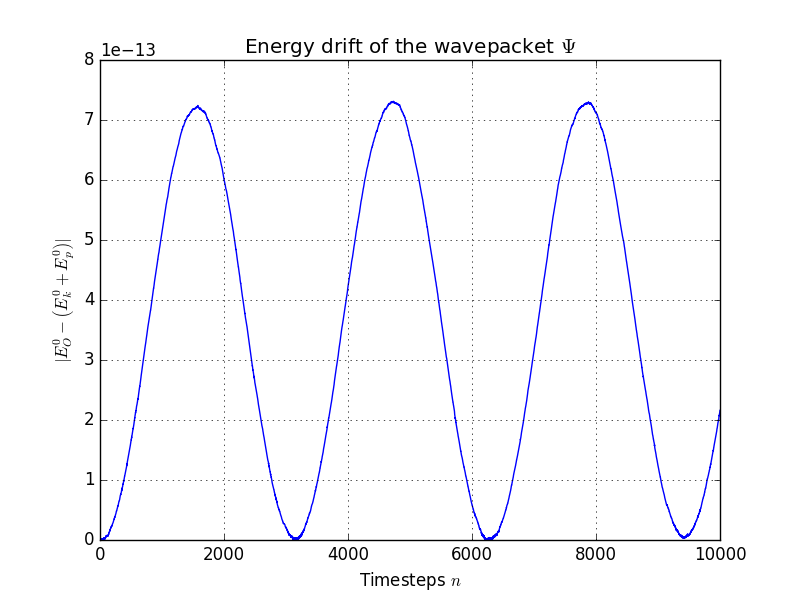
\includegraphics[width=.45\textwidth]{figures/harmonic_1D_Pre764_drift.png} \\
	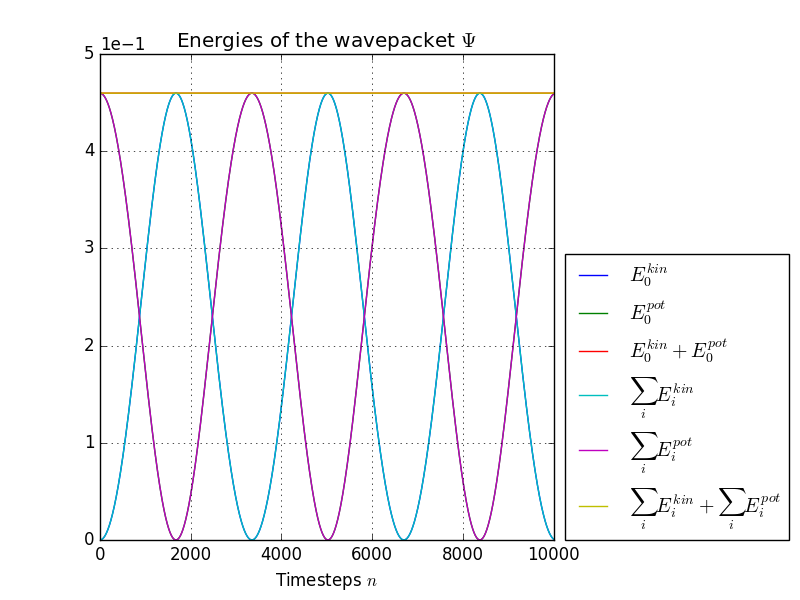
\includegraphics[width=.45\textwidth]{figures/torsional_1D_Pre764_energies.png}
	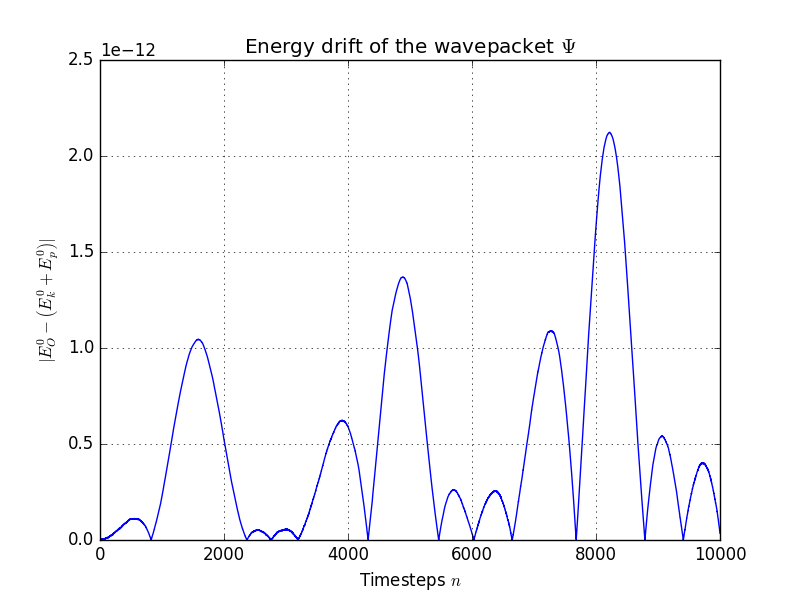
\includegraphics[width=.45\textwidth]{figures/torsional_1D_Pre764_drift.png} \\
	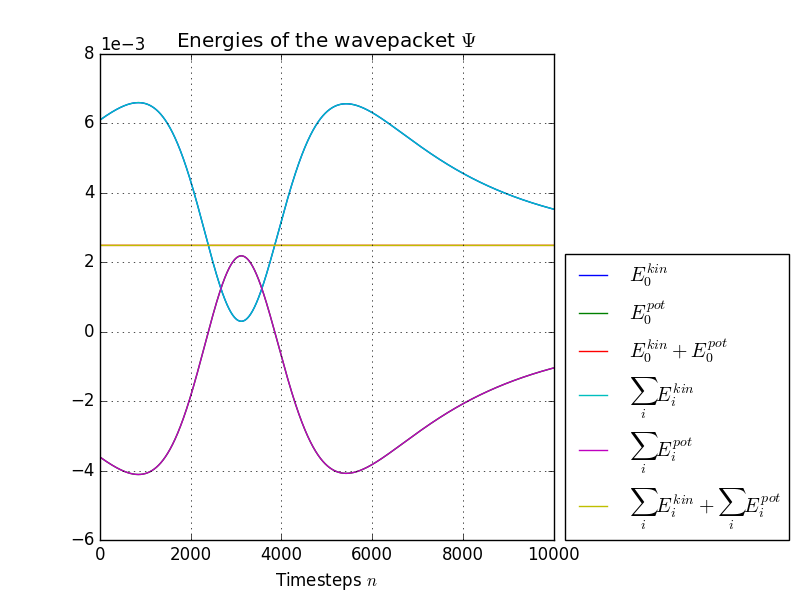
\includegraphics[width=.45\textwidth]{figures/morse_1D_Pre764_energies.png}
	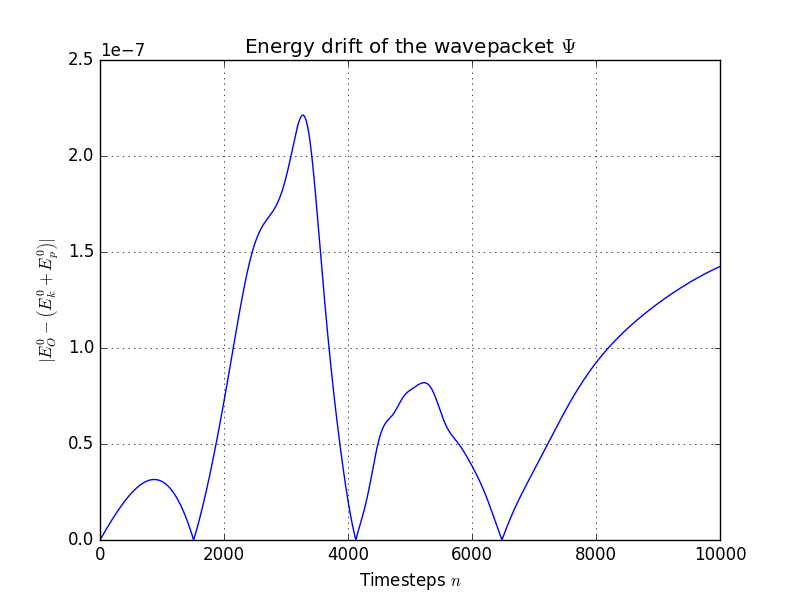
\includegraphics[width=.45\textwidth]{figures/morse_1D_Pre764_drift.png}
	\caption{Energy evolution and drift for a 1D wave packet propagated with the Pre764 propagator in a harmonic potential (top), a torsional potential (middle) and a Morse potential (bottom).
	(Parameters: $N=1$, $D=1$ $|\K|=16$ $\eps=0.01$ (Morse $0.0484$), $T=10$ (Morse $T=50$), $\Dt=0.001$ (Morse $\Dt=0.005$), Pre764 propagator with \emph{Y4} splitting for \proc{IntSplit})}
	\label{fig:energy_Pre764}
\end{figure}


\backmatter

\bibliographystyle{plain}
\bibliography{own,wp,references}

%\includepdf[pages={-}]{declaration-originality.pdf}

\end{document}
